\documentclass{article}
\usepackage{graphicx}
\usepackage{wrapfig}
\usepackage{subcaption}
\usepackage[margin=1in]{geometry}
\usepackage{amsmath} % or simply amstext
\usepackage{siunitx}
\usepackage{booktabs}
\usepackage[export]{adjustbox}
\newcommand{\angstrom}{\textup{\AA}}
\usepackage{cleveref}
\usepackage{booktabs}
\usepackage{gensymb}
\usepackage{float}

\title{Supplmental Information : Understanding the nanoscale structure of hexagonal phase lyotropic liquid crystal membranes}
\author{Benjamin J. Coscia \and Douglas L. Gin \and Richard D. Noble \and Joe Yelk \and Matthew Glaser \and Xunda Feng \and Michael R. Shirts}

\begin{document}

  \graphicspath{{./figures/}}  % put all the figures here
  \maketitle

  \begin{figure}
        \centering
        \begin{subfigure}[b]{0.32\textwidth}
                \centering
                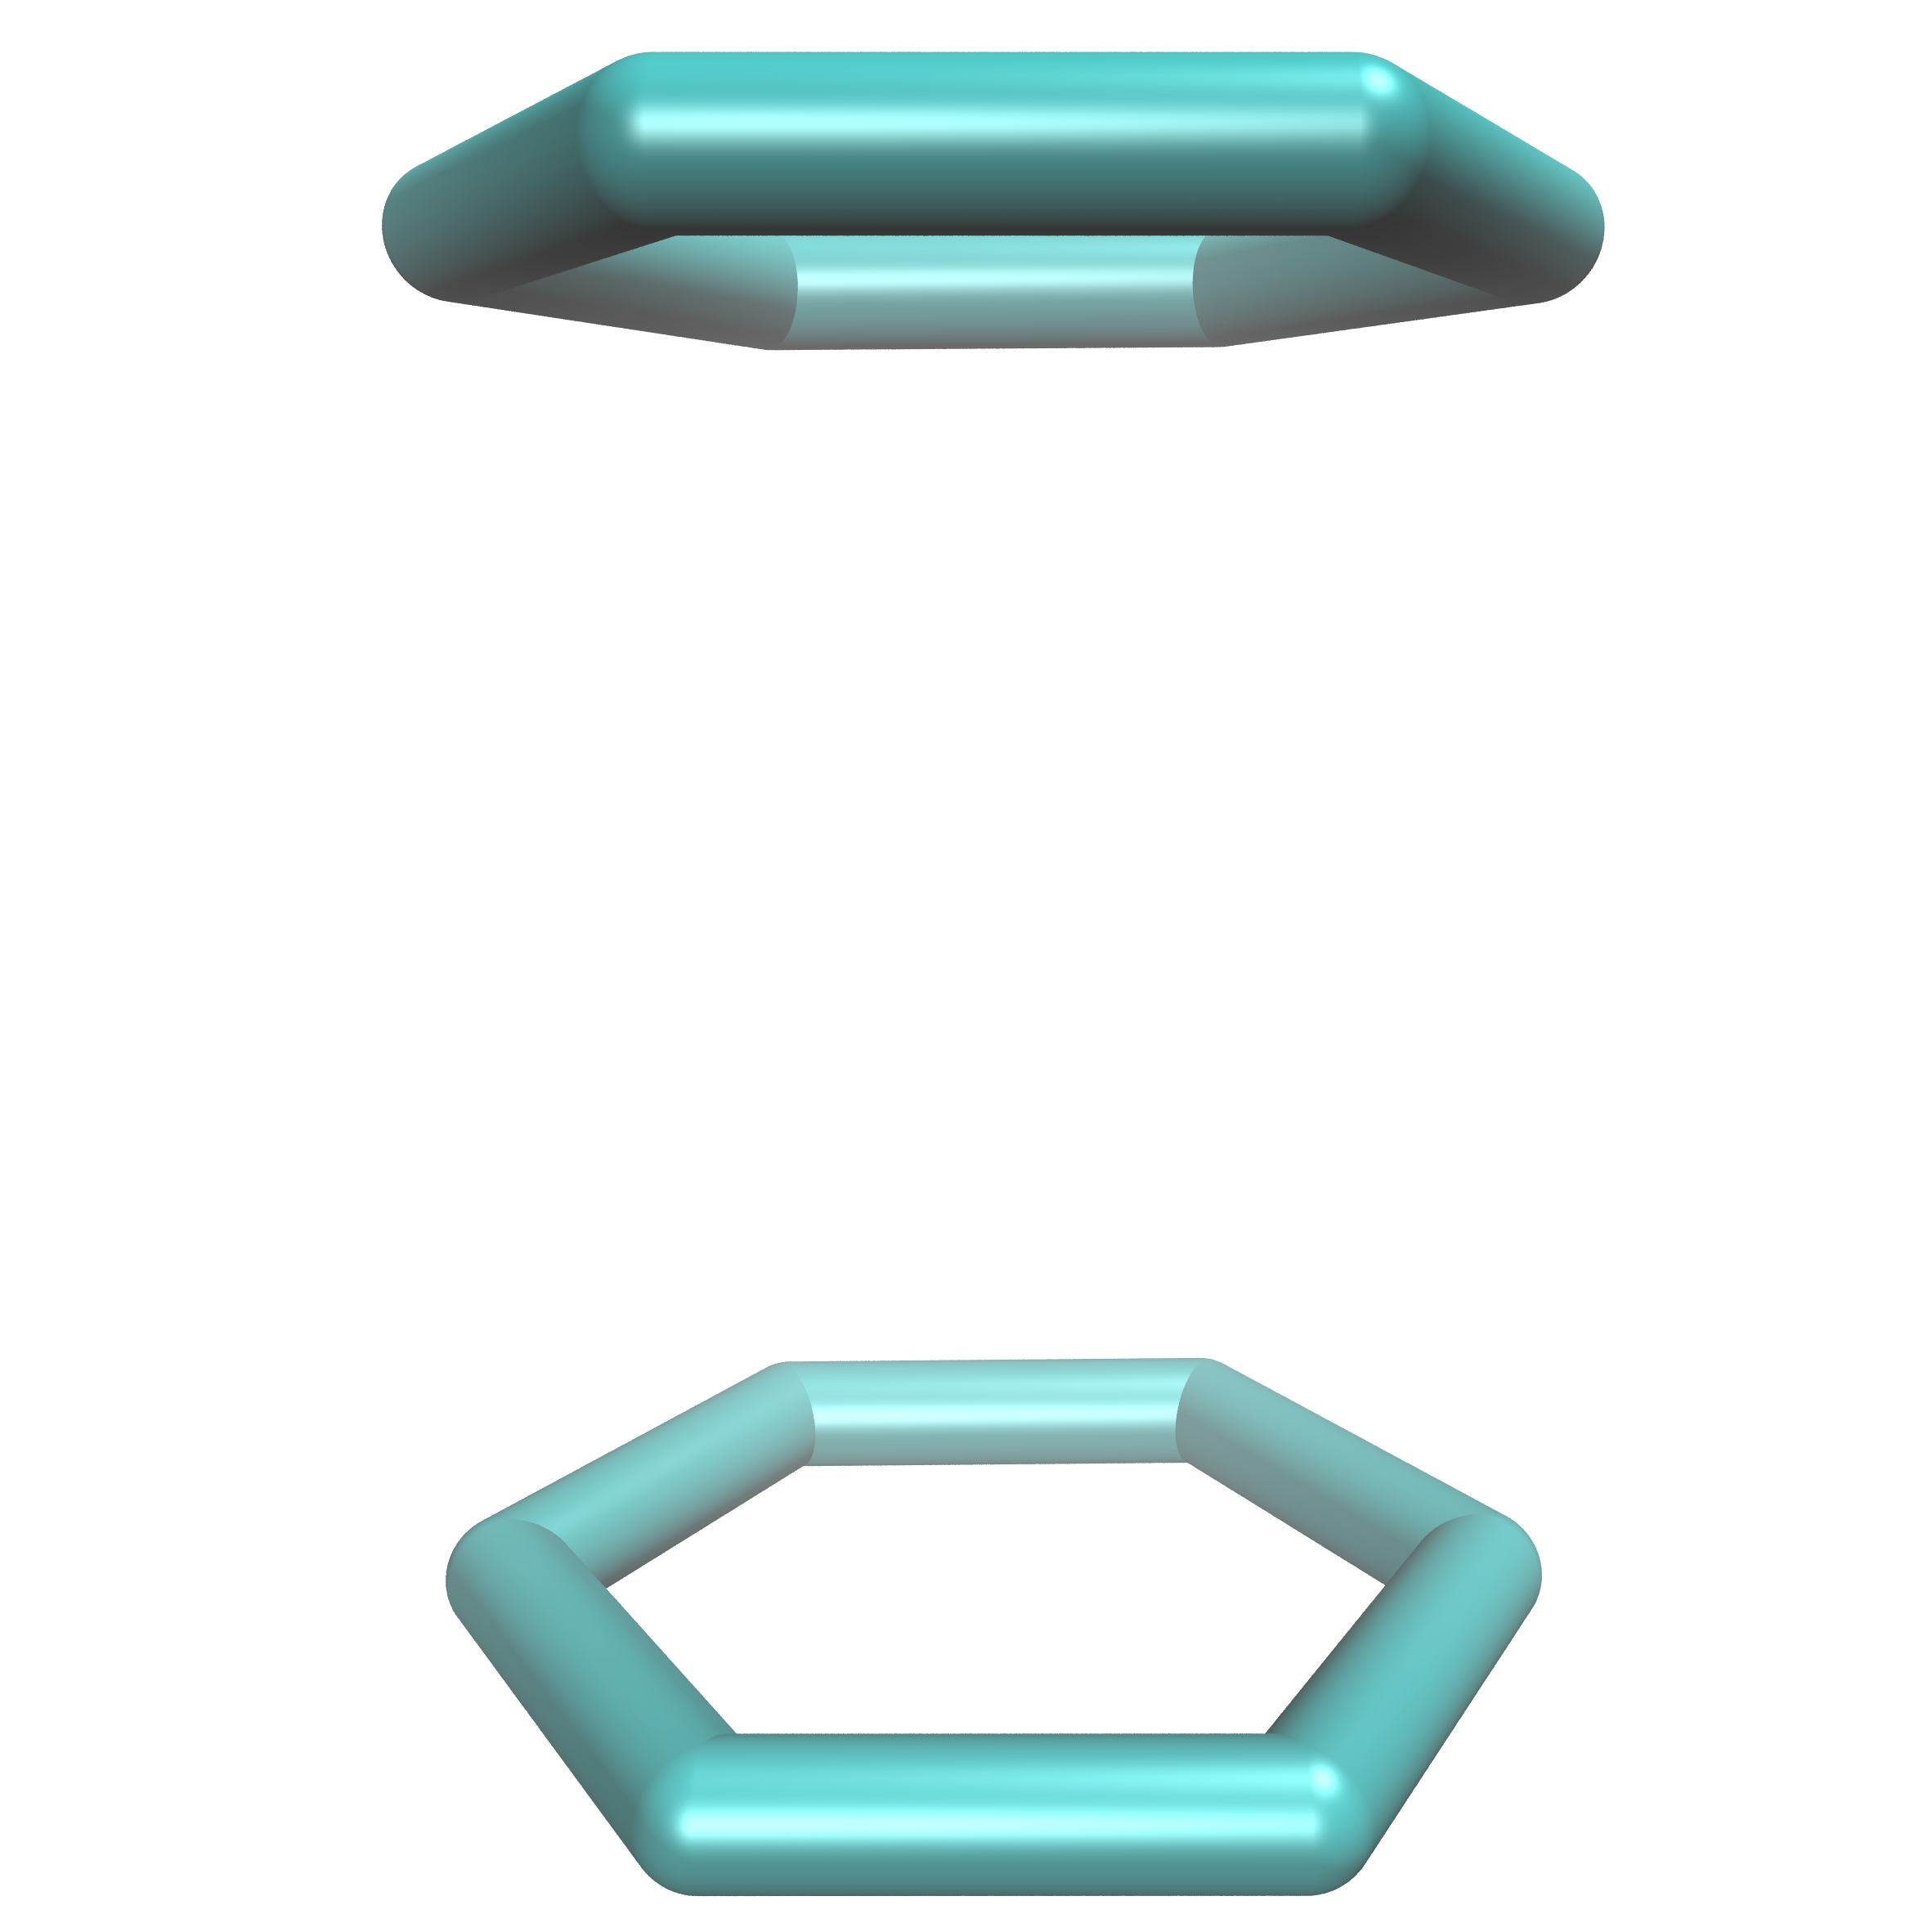
\includegraphics[width=\textwidth]{sandwiched.png}
                \caption{}\label{fig:sandwiched}
        \end{subfigure}
        \begin{subfigure}[b]{0.32\textwidth}
                \centering
                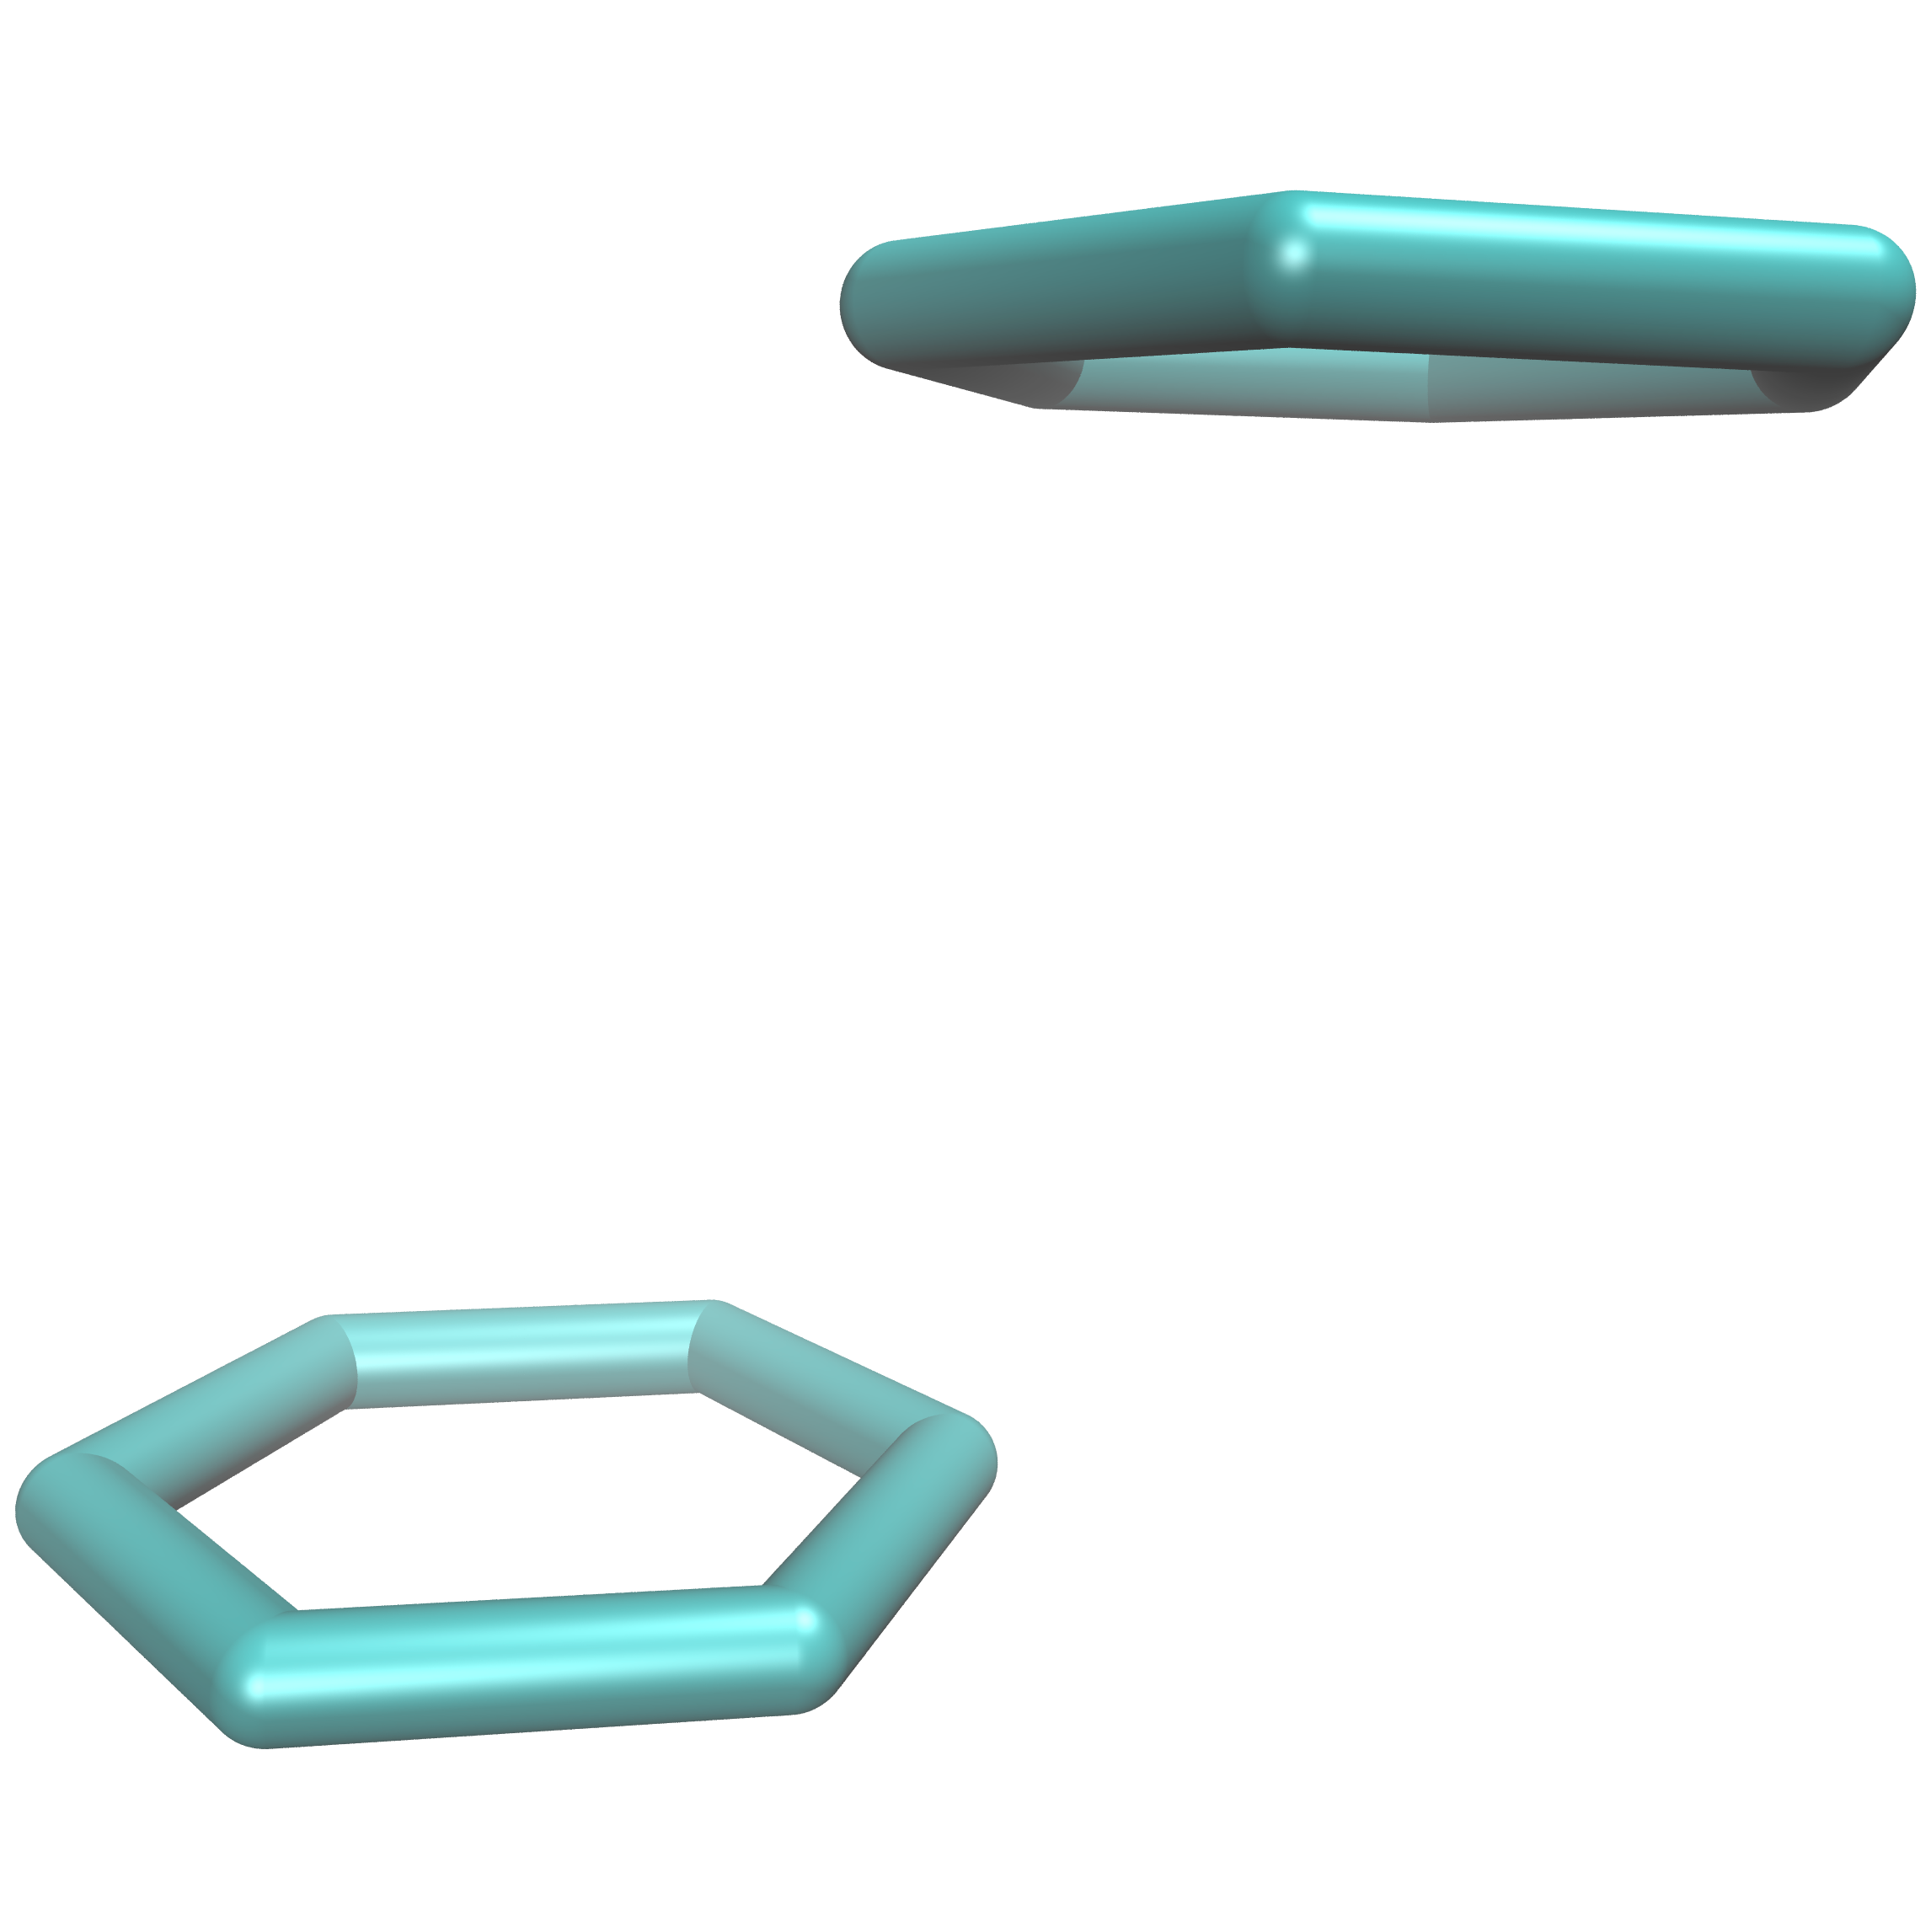
\includegraphics[width=\textwidth]{PD.png}
                \caption{}\label{fig:pd}
        \end{subfigure}
        \begin{subfigure}[b]{0.32\textwidth}
                \centering
                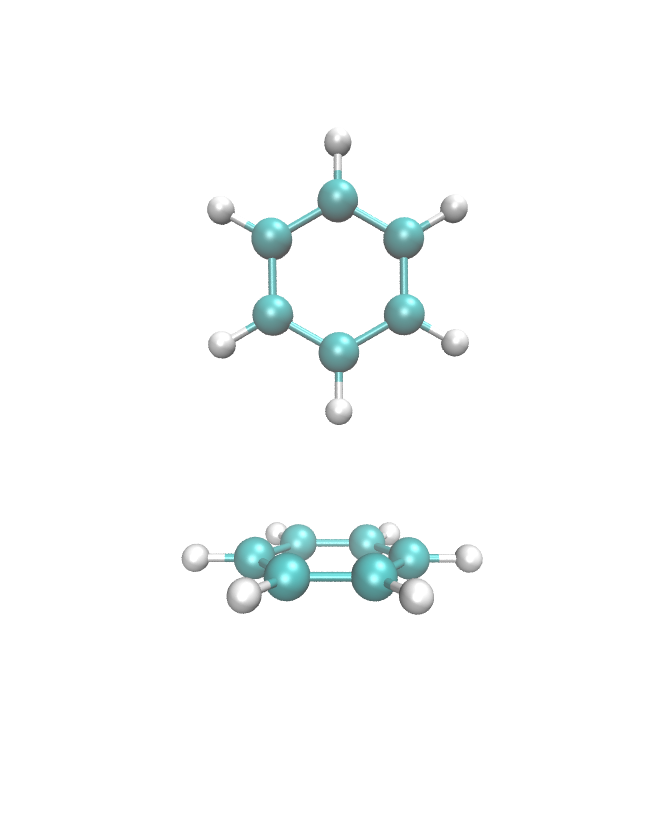
\includegraphics[width=\textwidth]{Tshaped.png}
                \caption{}\label{fig:tshaped}
        \end{subfigure}
        \vskip\baselineskip
        \begin{subfigure}[b]{0.475\textwidth}
                \centering
                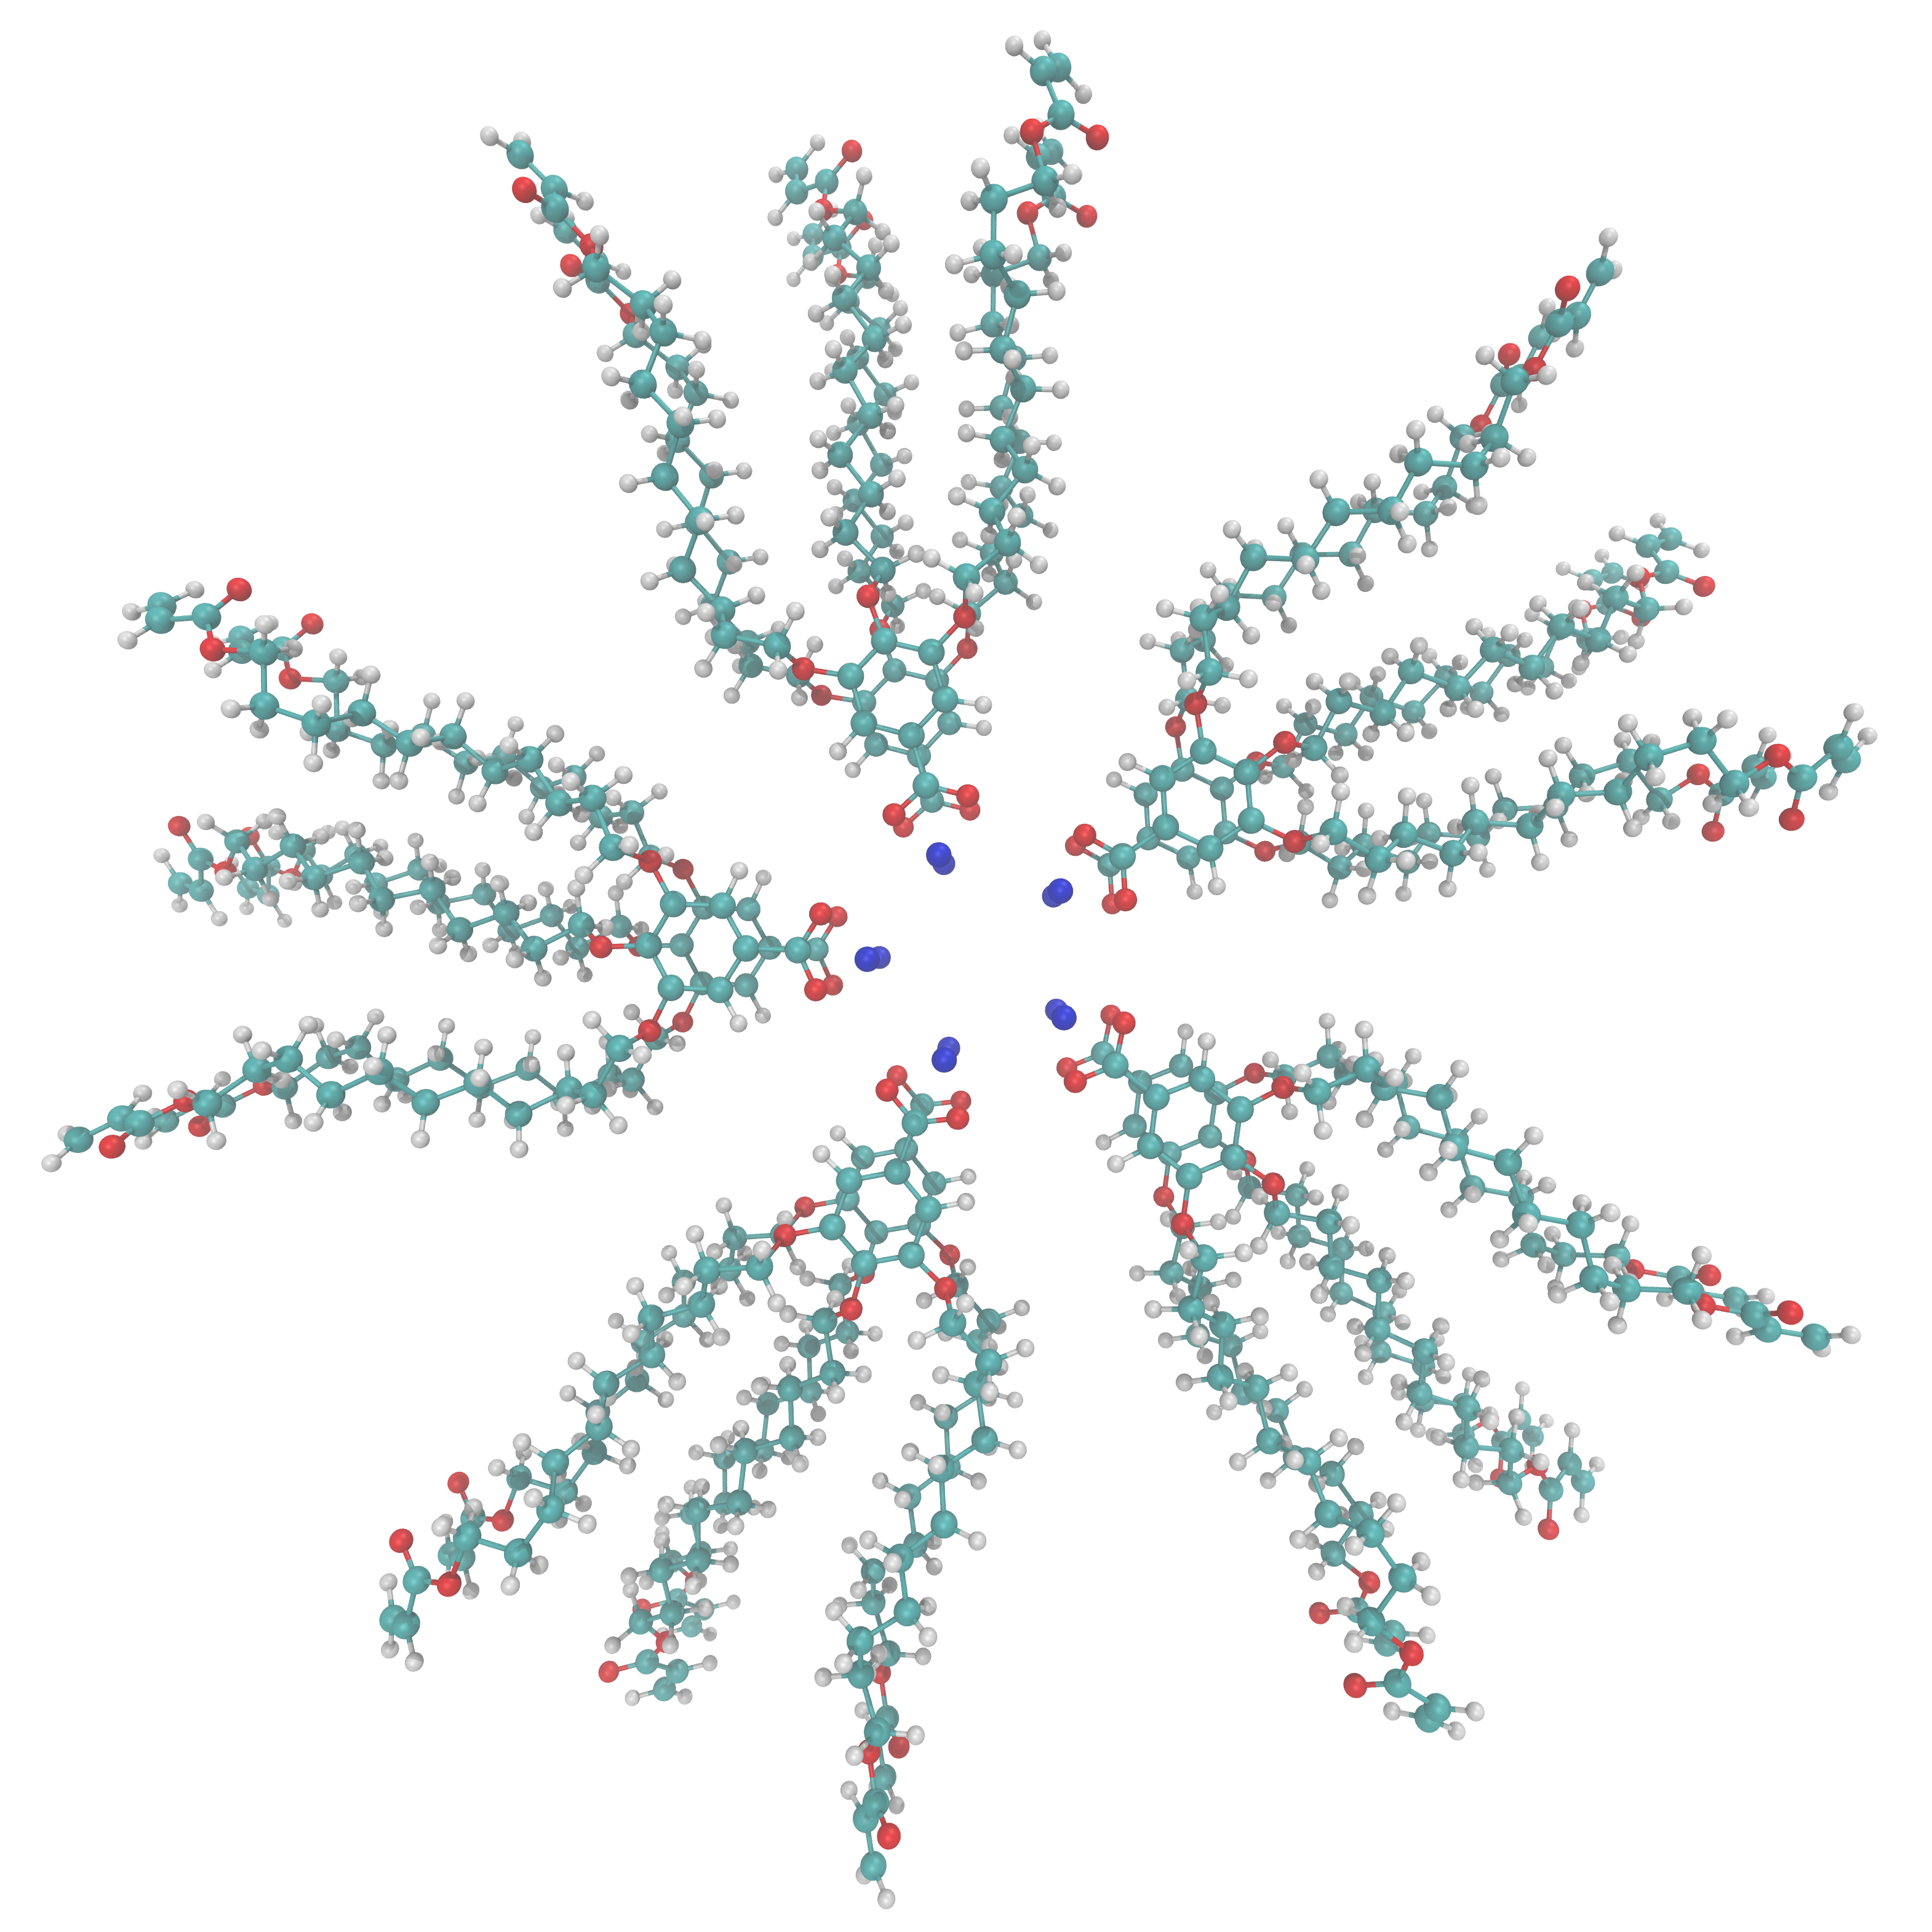
\includegraphics[width=\textwidth]{sandwichedlayers.png}
                \caption{}\label{fig:sandwichedlayers}
        \end{subfigure}
        \begin{subfigure}[b]{0.475\textwidth}
                \centering
                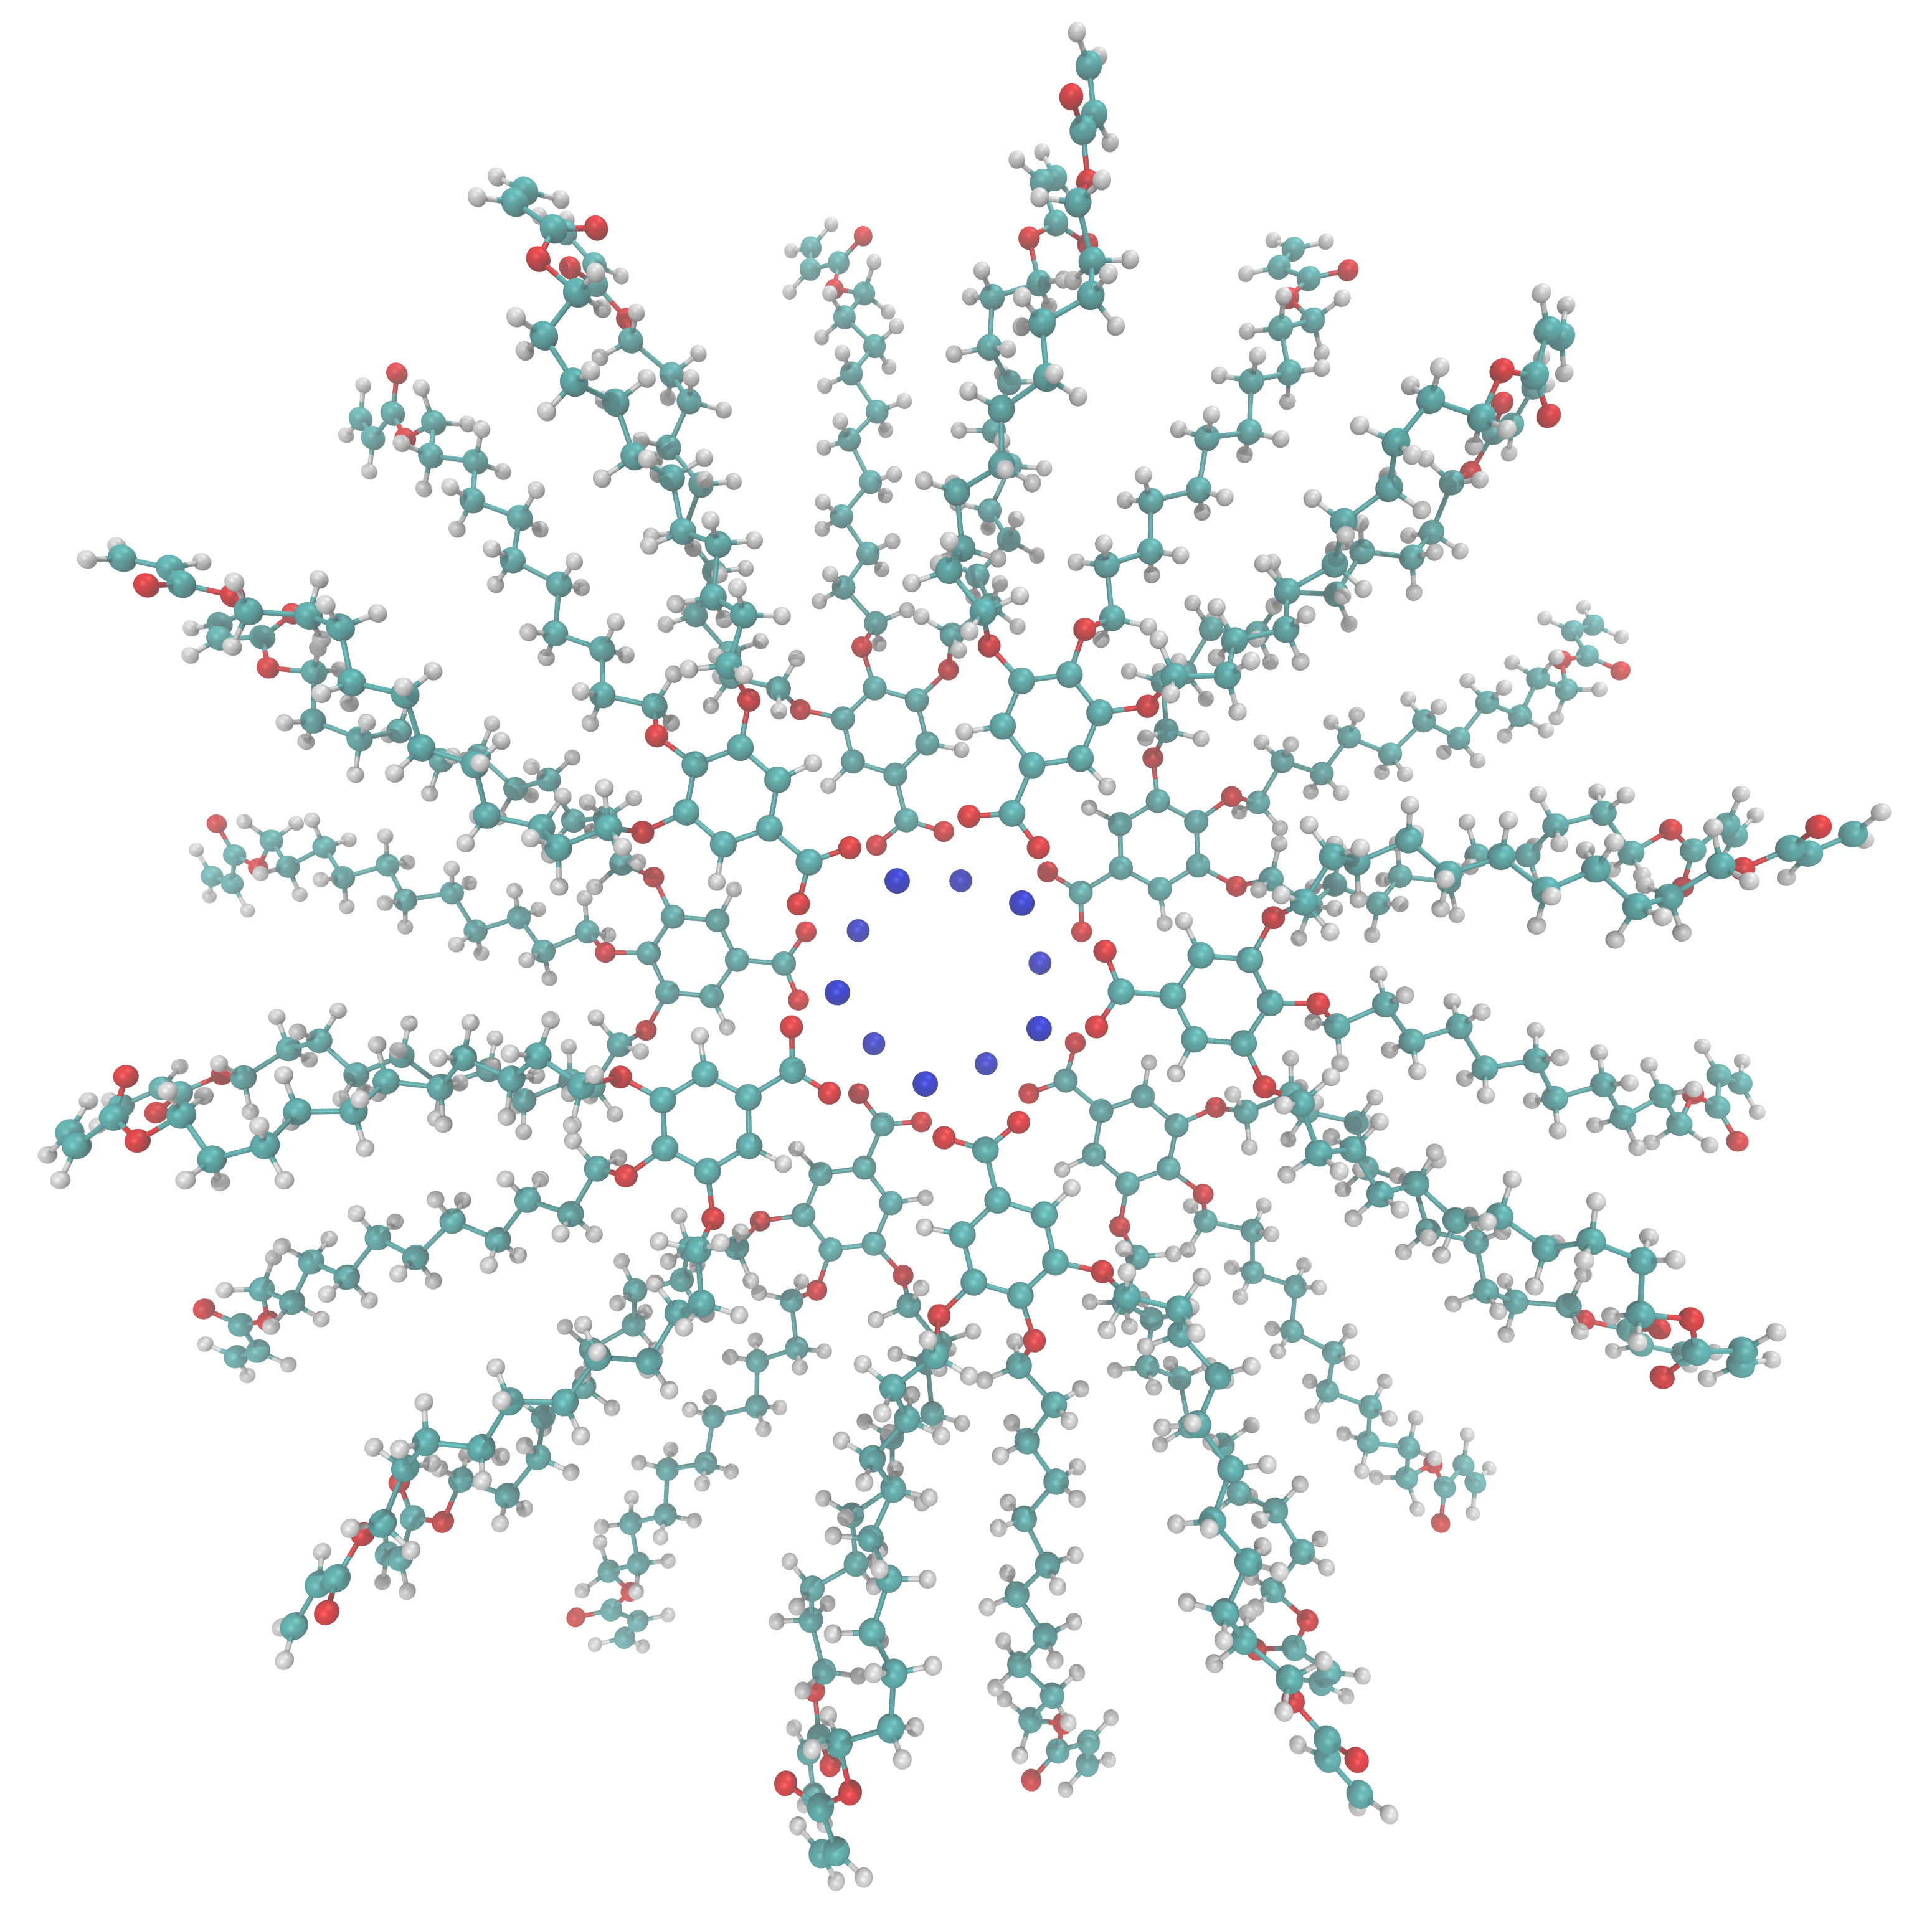
\includegraphics[width=\textwidth]{offsetlayers.png}
                \caption{}\label{fig:offsetlayers}
        \end{subfigure}
        \caption{(a) Sandwiched benzene dimers stack 3.8 \angstrom~apart. (b) Parallel-Displaced benzene dimers stack
        3.4 \angstrom~vertically and 1.6 \angstrom~horizontally apart. (c) T-shaped benzene dimers stack 5.0 \angstrom~apart.
        (d) Two monomer layers stacked in the sandwiched configuration (e) Two monomer layers stacked in the parallel-displaced
        configuration }\label{fig:stacking}
  \end{figure}

  \begin{figure}
	\centering
        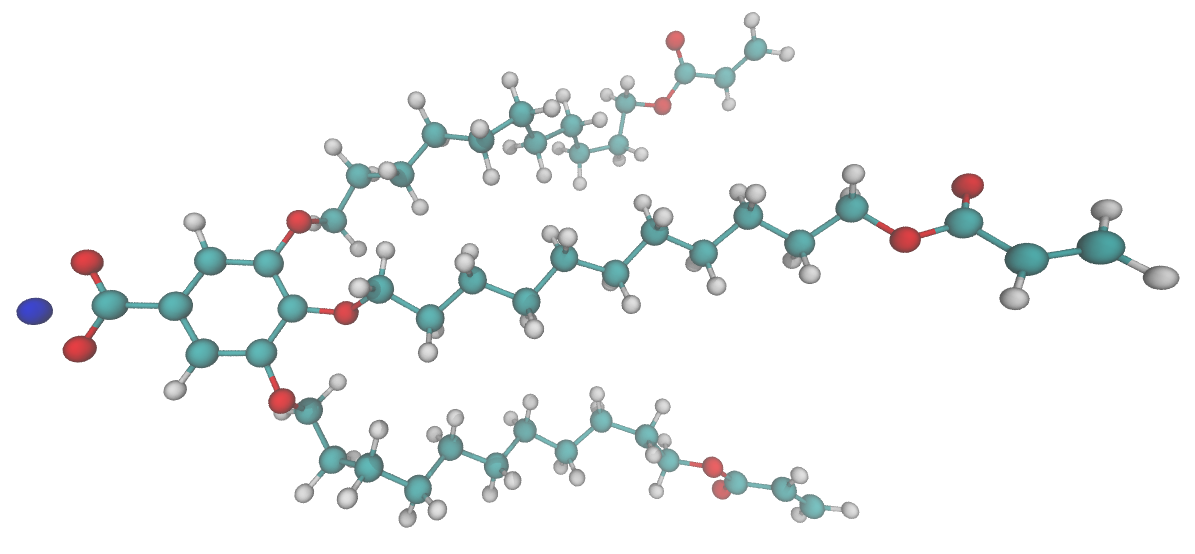
\includegraphics[width=0.9\textwidth]{monomer.png}
	\caption{Atomistic representation of the monomer Na-GA3C11. White atoms
		represent hydrogen, cyan atoms represent carbon, red atoms represent oxygen and
		the blue atom is sodium.}\label{fig:monomer}
  \end{figure}

  \begin{figure}
	\centering
        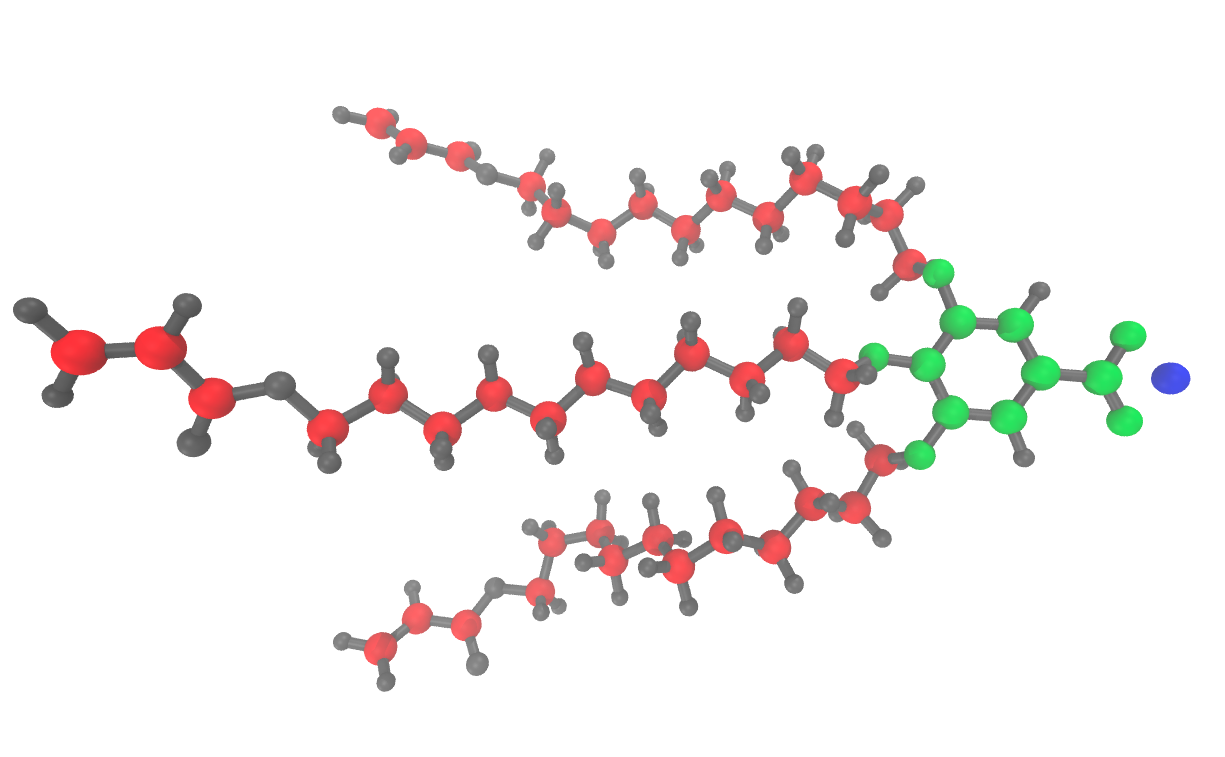
\includegraphics[width=0.9\textwidth]{monomer_color_coded.png}
	\caption{The groups used for $g(z)$ calculations. Red atoms are in the
		tails group. Green atoms are in the head group region. The blue atom is sodium. 
		}\label{fig:monomer_color_coded}
  \end{figure}

  \begin{figure}
	\centering
	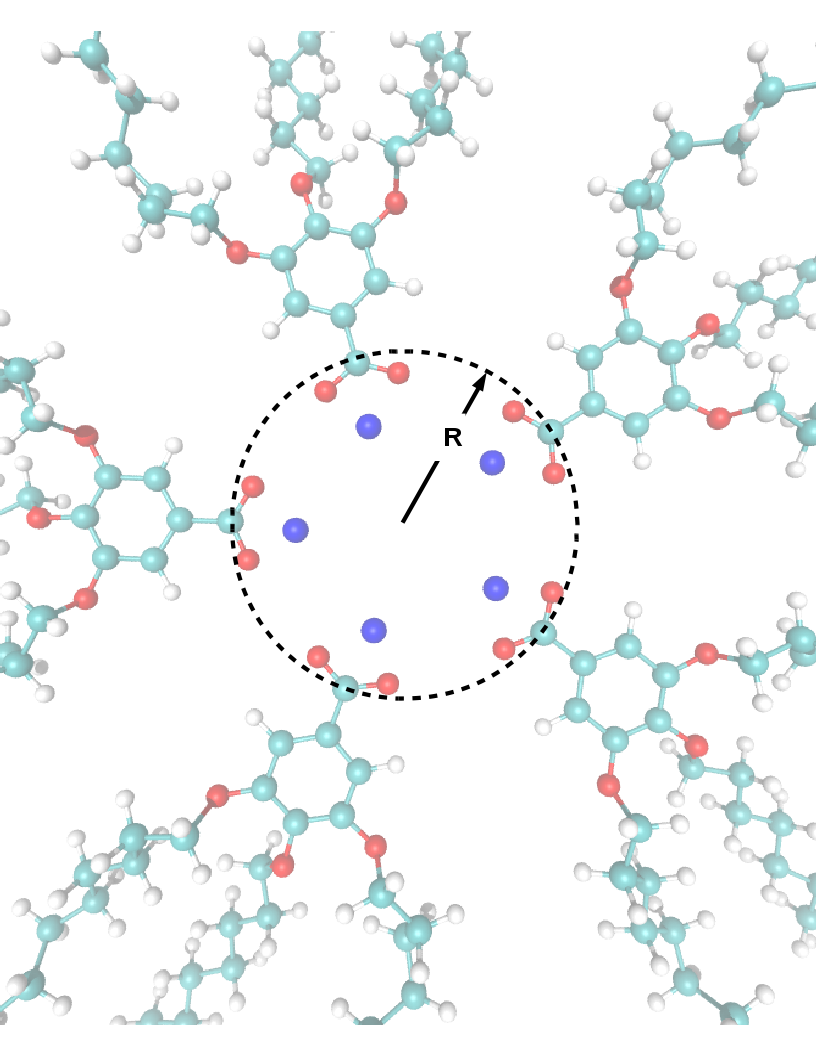
\includegraphics[width=0.8\textwidth]{pore_radius_illustration.png}
	\caption{When creating an initial configuration, the pore radius is defined based
	on the distance of the carbonyl carbon from the pore's central axis}
	\label{fig:pore_radius_illustration}
  \end{figure}

  \textbf{TODO} : These are things I am working on / need to do

  \begin{itemize}
  \item Initial configuration dependence
	\begin{itemize}
		\item Initial pore-to-pore spacing
		\item Initial pore radius
		\item I have simulations running to support the claims that
		these are not significant factors if chosen within reason. And
		I will define what is meant by 'within reason'.
	\end{itemize}
  \item Description of parameterization process
  \item Feel free to suggest anything else that might be useful
  \end{itemize}
 

  \textbf{Calculation of pore-to-pore spacing statistics}
  
  \color{red}{This is an outline of this section and will be reworded for clarity}
  \begin{itemize}
  \item We are interested in 5 pore-to-pore distances which should all be equal
  in a perfect hexagonal array, however only 4 distances are independent % can
  visualize this in supplemental material. Will make a lot of things more clear
  below.
  \item Each pore spacing has its own trajectory of spacing vs. time. Using
  data collected after the system is equilibrated, we calculate how long it takes
  for the data in each of the 5 trajetories to become uncorrelated using
  pymbar.timeseries.integratedAutocorrelationTime() % reference
  \item We break the full trajectories down into sub-trajectories based on the
  maximum autocorrelation time of those found in the previous step.
  \item For each bootstrap trial, we recreate an equilibrium trajectory by
  randomly sampling pore spacings from the sub-trajectories 
  \item We get an average value for each pore spacing by finding the mean of
  the bootstrapped data
  \item We calculate the overall average as the mean of all bootstrapped pore
  spacings
  \item The uncertainty for each pore spacing is calculated as $\dfrac{<x> -
  x}{4}$ where $<x>$ is the average spacing from the bootstrap trial and $x$ is
  the average value of one of the pore spacings.
  \item We report the mean of these uncertainties
  \end{itemize}

  \begin{figure}
	\centering
        \begin{subfigure}{0.40\textwidth}
                \centering
                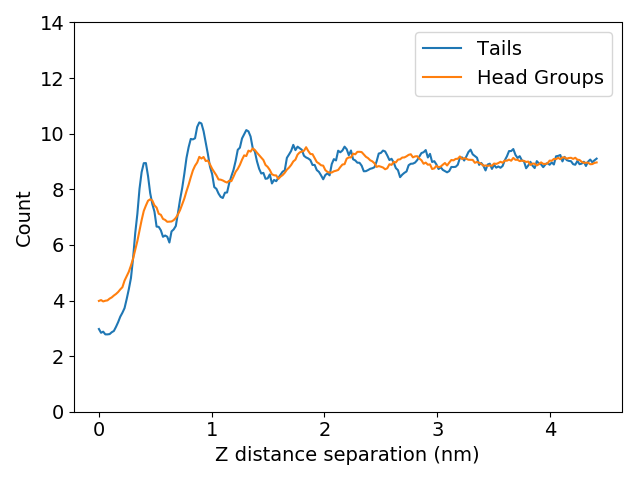
\includegraphics[width=\textwidth]{zdf_layered_4.png}
                \caption{4 mon/layer, Sandwiched}\label{fig:zdf_layered_4}
        \end{subfigure}
        \begin{subfigure}{0.40\textwidth}
                \centering
                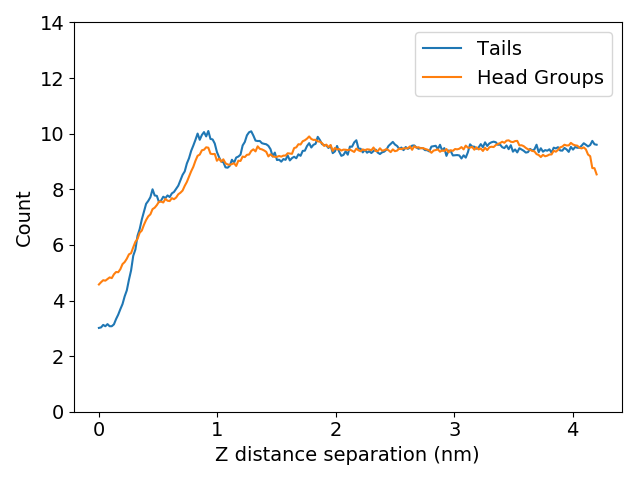
\includegraphics[width=\textwidth]{zdf_offset_4.png}
                \caption{4 mon/layer, Parallel Displaced}\label{fig:zdf_layered_4}
        \end{subfigure}
	\begin{subfigure}{0.40\textwidth}
                \centering
                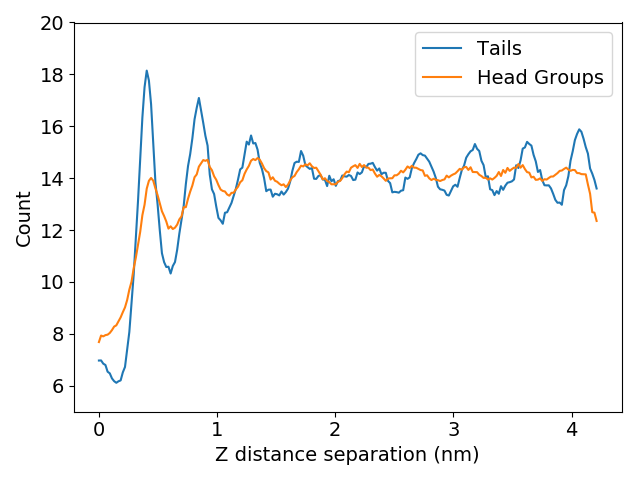
\includegraphics[width=\textwidth]{zdf_layered_6.png}
                \caption{6 mon/layer, Sandwiched}\label{fig:zdf_layered_6}
        \end{subfigure}
        \begin{subfigure}{0.40\textwidth}
                \centering
                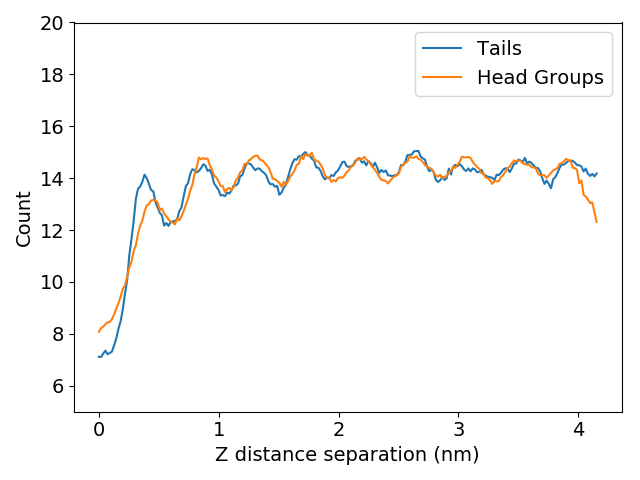
\includegraphics[width=\textwidth]{zdf_offset_6.png}
                \caption{6 mon/layer, Parallel Displaced}\label{fig:zdf_layered_6}
        \end{subfigure}
        \begin{subfigure}{0.40\textwidth}
                \centering
                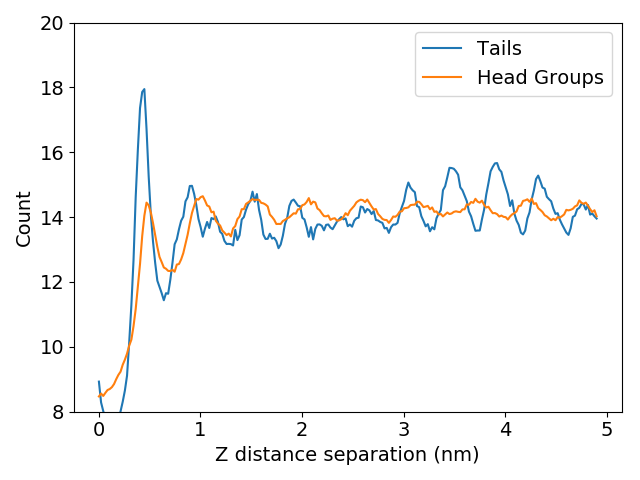
\includegraphics[width=\textwidth]{zdf_layered_7.png}
                \caption{7 mon/layer, Sandwiched}\label{fig:zdf_layered_7}
        \end{subfigure}
        \begin{subfigure}{0.40\textwidth}
                \centering
                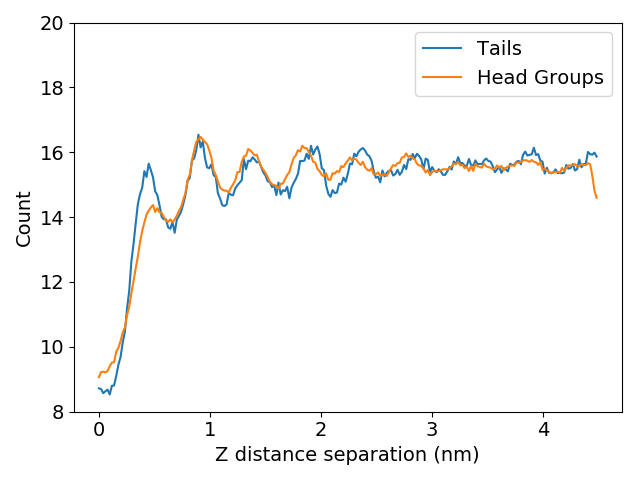
\includegraphics[width=\textwidth]{zdf_offset_7.png}
                \caption{7 mon/layer, Parallel Displaced}\label{fig:zdf_layered_7}
        \end{subfigure}
	\begin{subfigure}{0.40\textwidth}
                \centering
                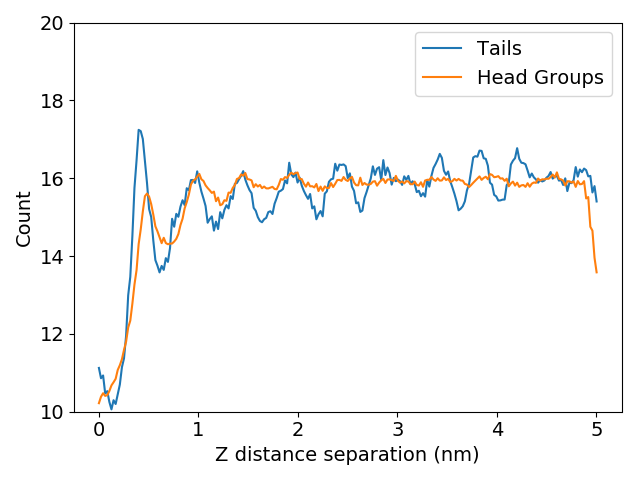
\includegraphics[width=\textwidth]{zdf_layered_8.png}
                \caption{8 mon/layer, Sandwiched}\label{fig:zdf_layered_8}
        \end{subfigure}
        \begin{subfigure}{0.40\textwidth}
                \centering
                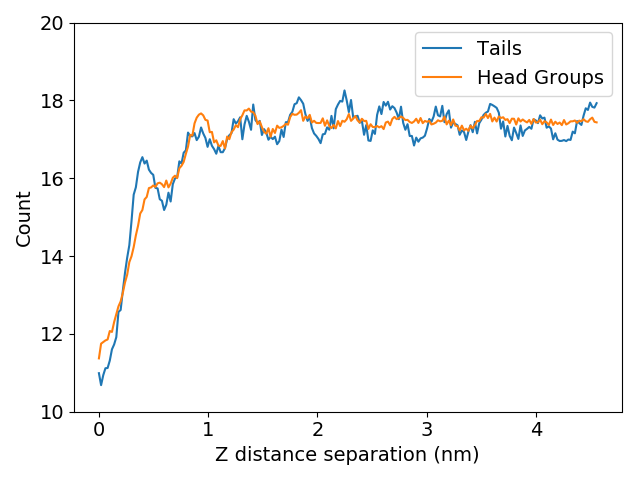
\includegraphics[width=\textwidth]{zdf_offset_8.png}
                \caption{8 mon/layer, Parallel Displaced}\label{fig:zdf_layered_8}
        \end{subfigure}
	\caption{$g(z)$ for all other configurations built with layers stacked 3.7 \AA~apart}\label{fig:zdf}
  \end{figure}

  \begin{figure}
	\centering
        \begin{subfigure}{0.40\textwidth}
                \centering
                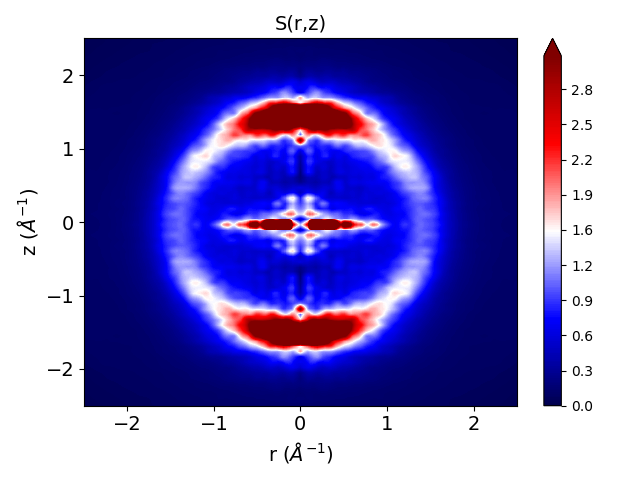
\includegraphics[width=\textwidth]{rzplot_layered_4.png}
                \caption{4 mon/layer, Sandwiched}\label{fig:rzplot_layered_4}
        \end{subfigure}
        \begin{subfigure}{0.40\textwidth}
                \centering
                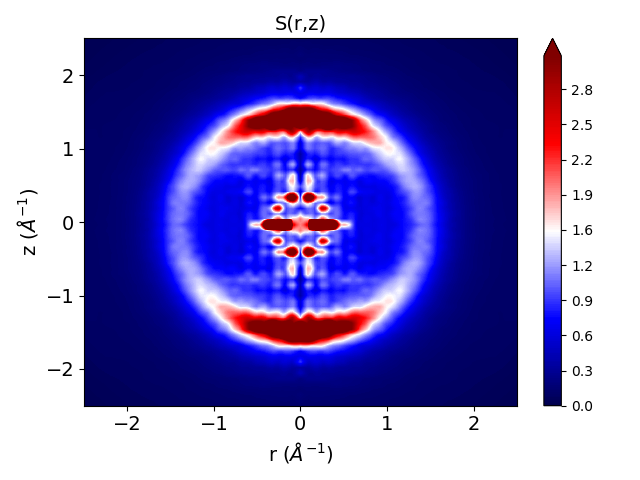
\includegraphics[width=\textwidth]{rzplot_offset_4.png}
                \caption{4 mon/layer, Parallel Displaced}\label{fig:rzplot_offset_4}
        \end{subfigure}
        \begin{subfigure}{0.40\textwidth}
                \centering
                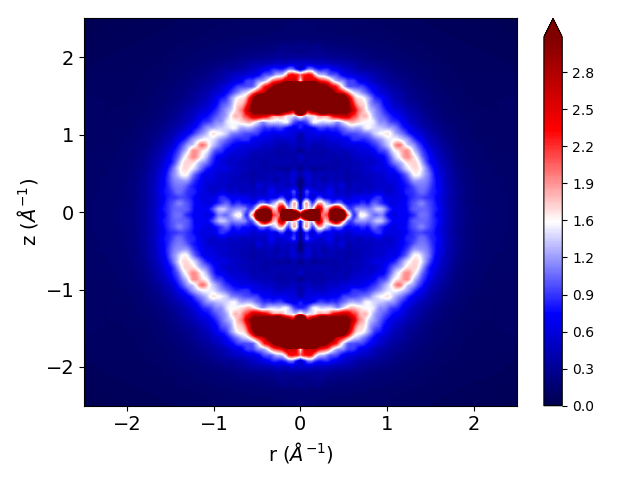
\includegraphics[width=\textwidth]{rzplot_layered_6.png}
                \caption{6 mon/layer, Sandwiched}\label{fig:rzplot_layered_6}
        \end{subfigure}
        \begin{subfigure}{0.40\textwidth}
                \centering
                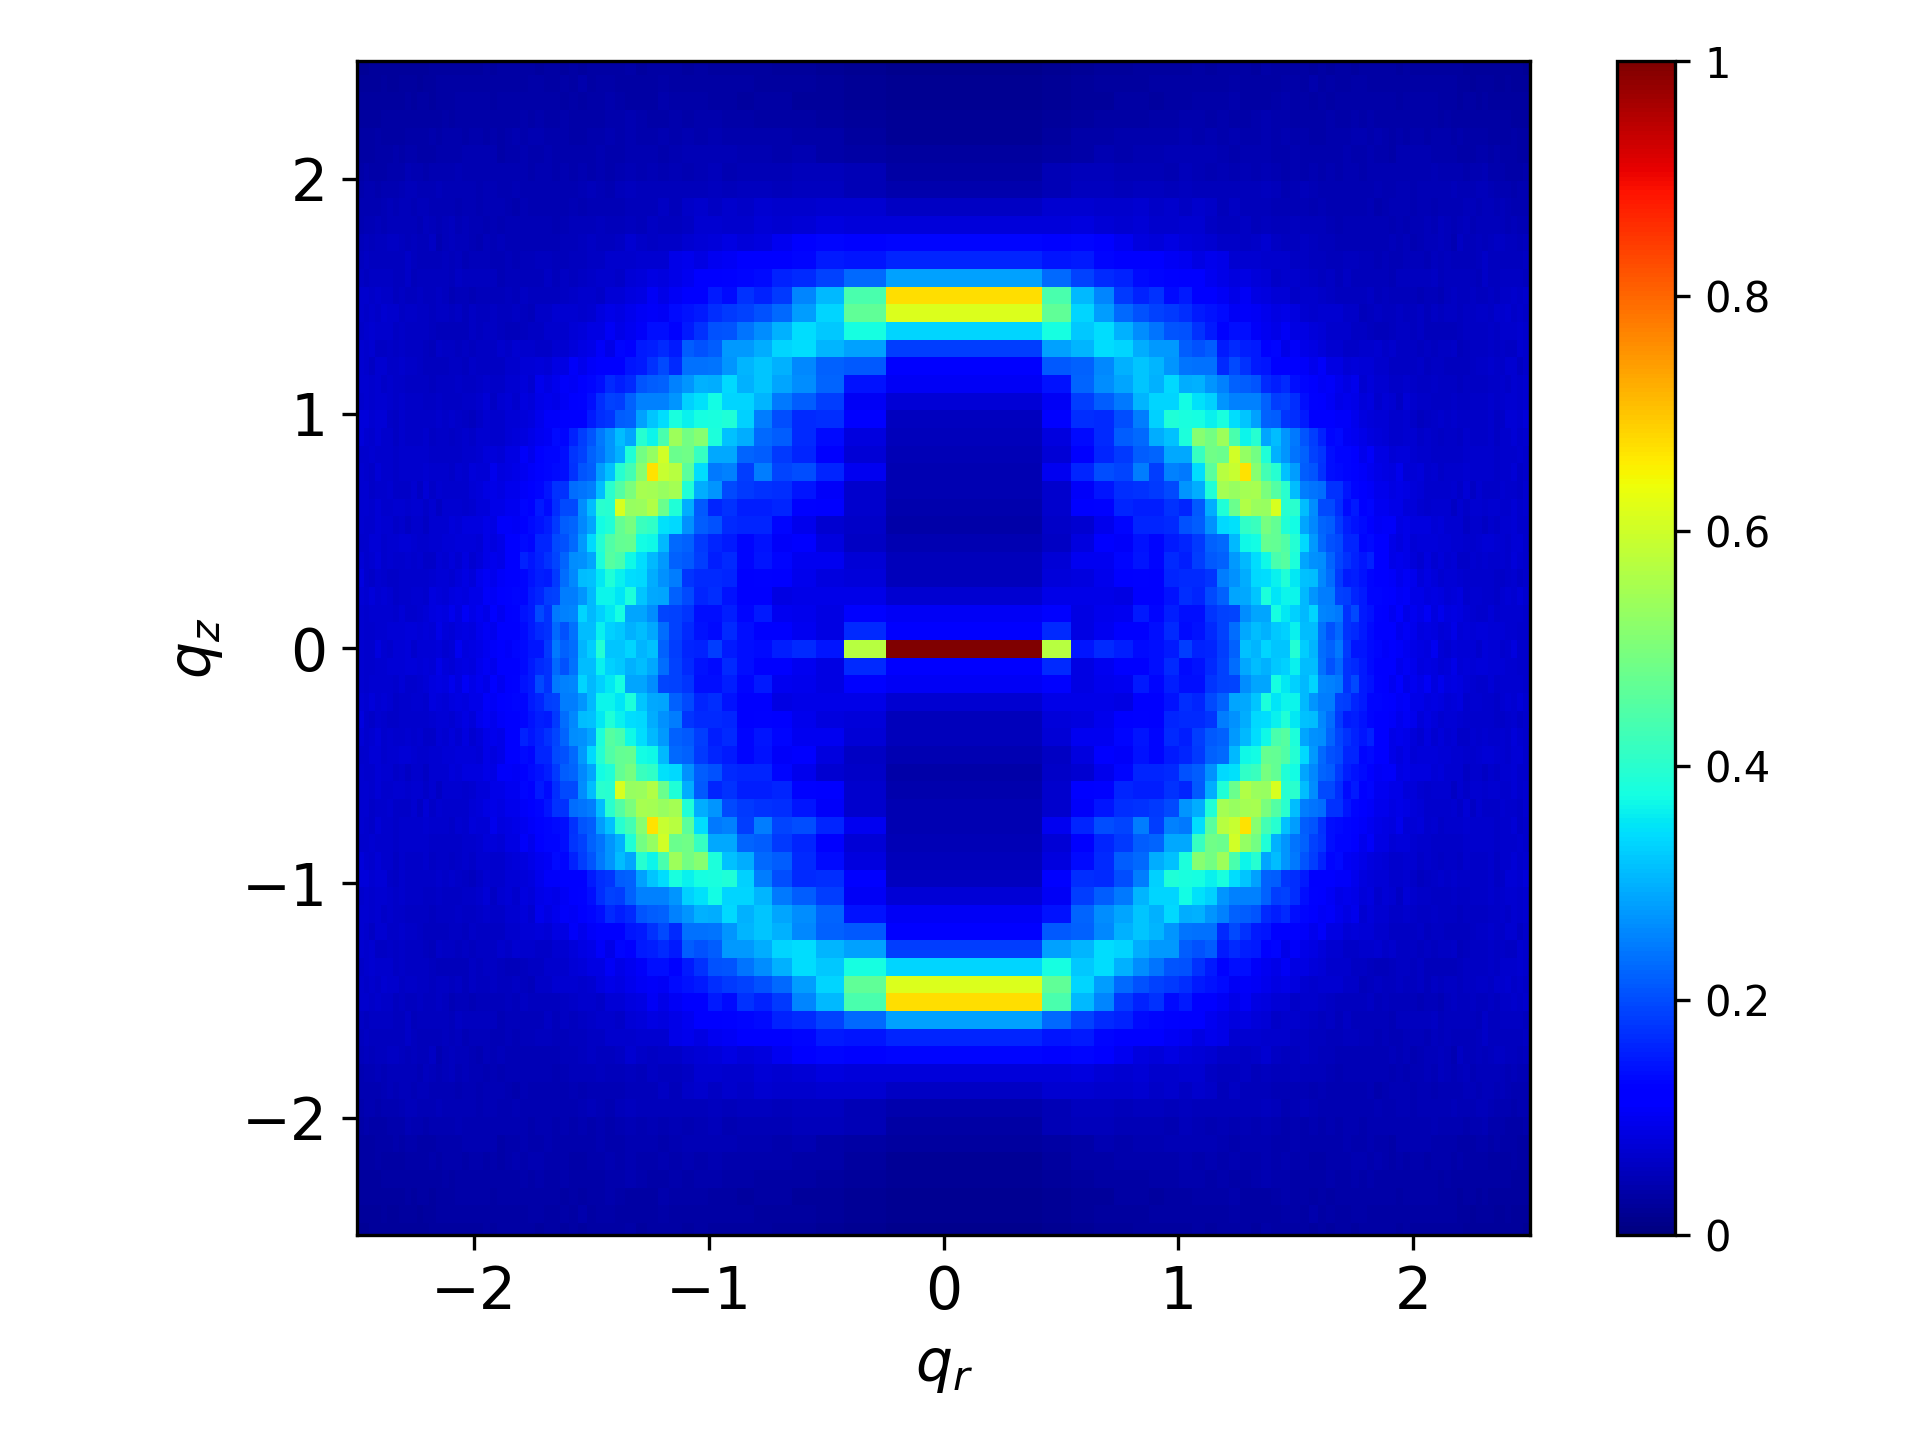
\includegraphics[width=\textwidth]{rzplot_offset_6.png}
                \caption{6 mon/layer, Parallel Displaced}\label{fig:rzplot_offset_6}
        \end{subfigure}
        \begin{subfigure}{0.40\textwidth}
                \centering
                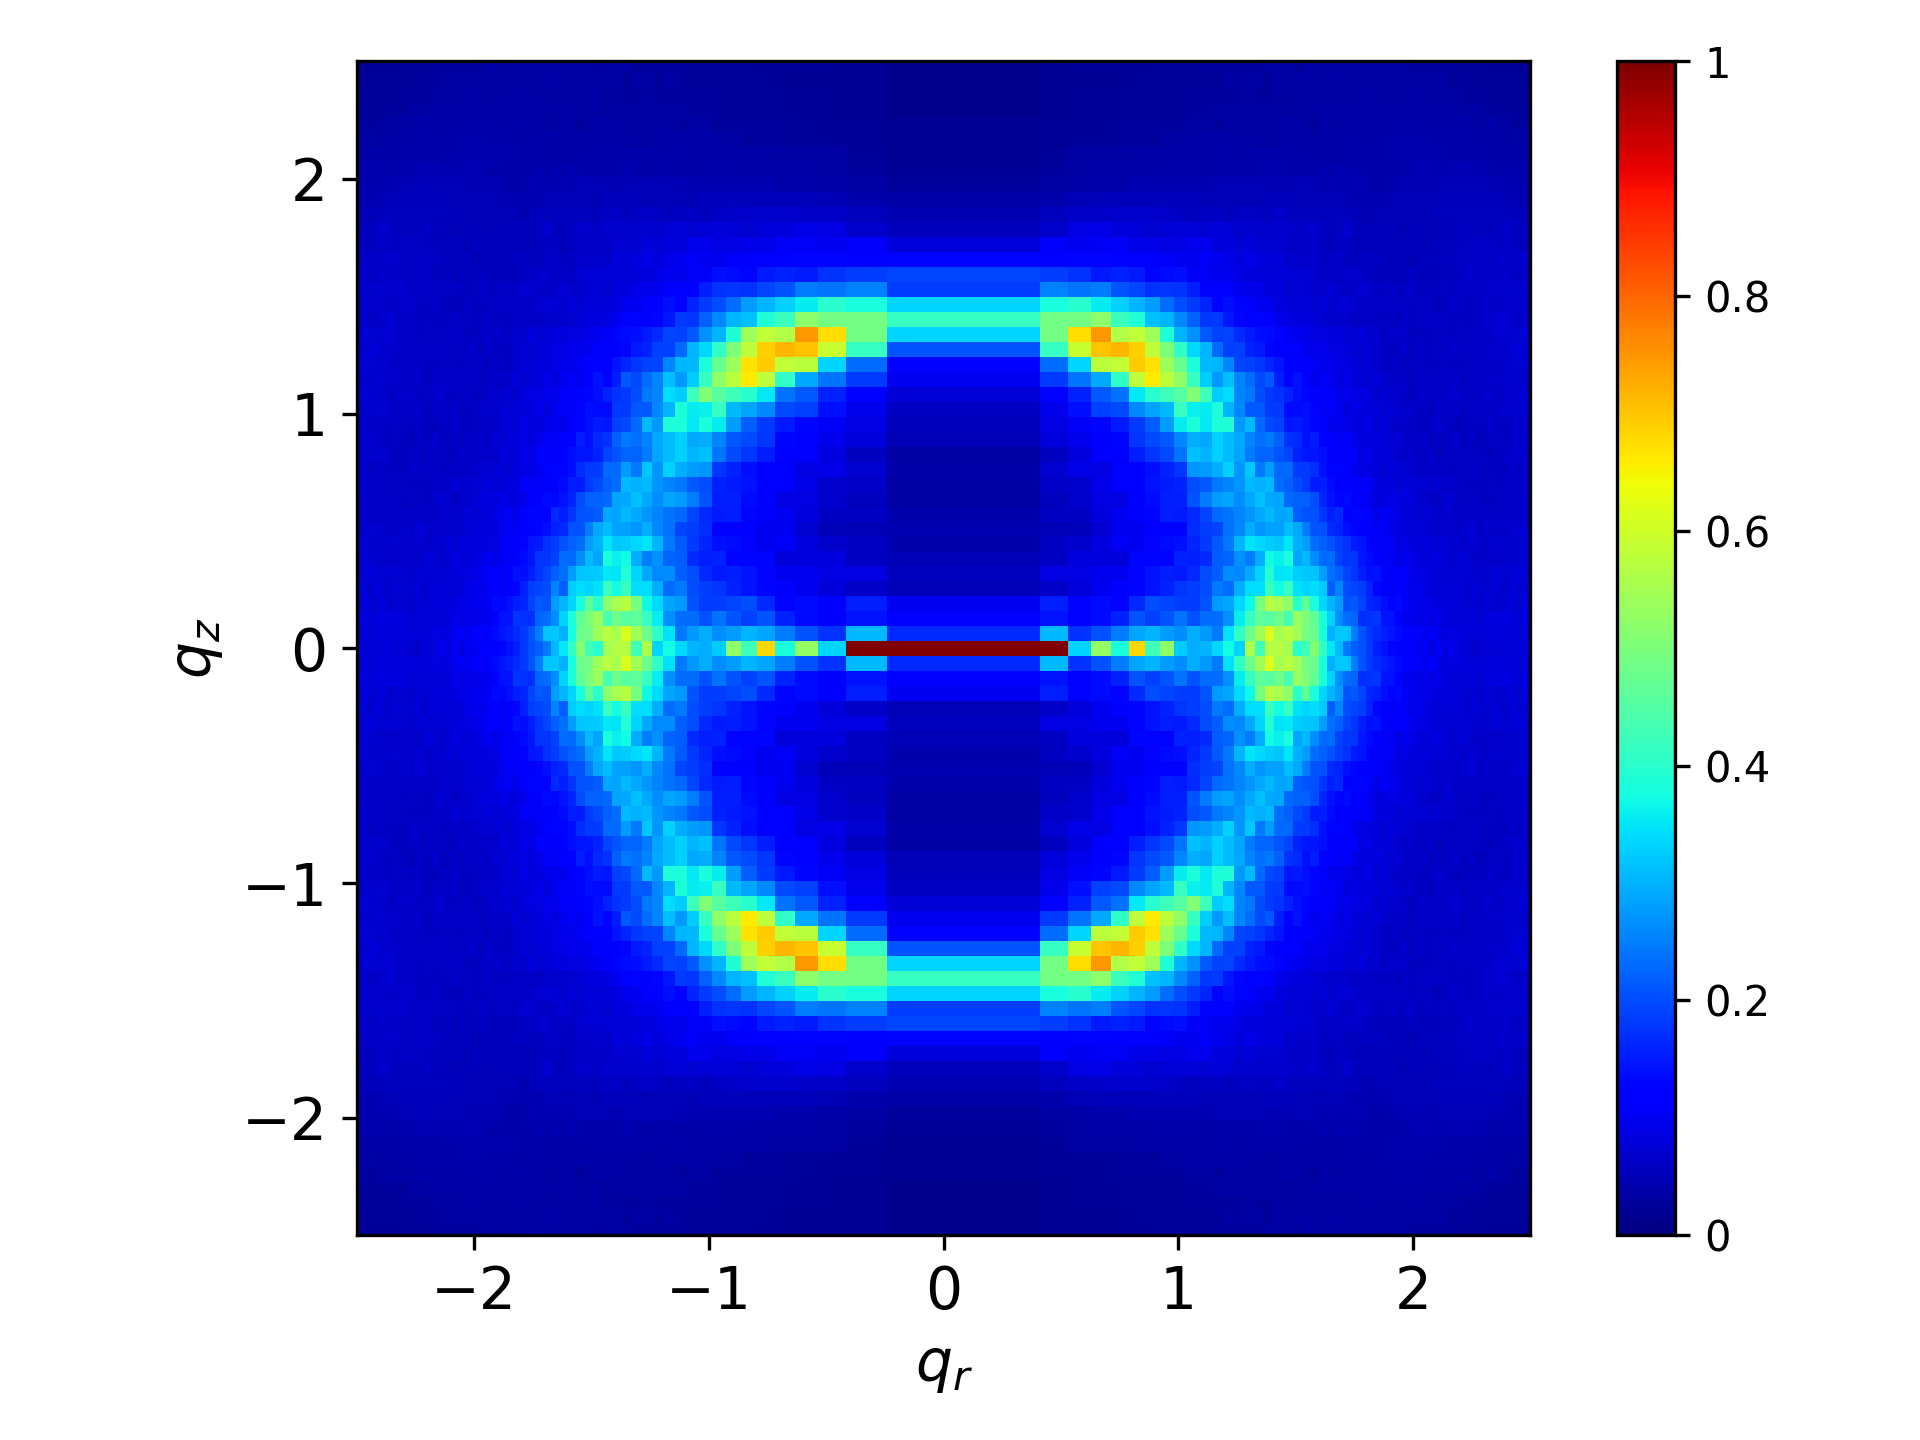
\includegraphics[width=\textwidth]{rzplot_layered_7.png}
                \caption{7 mon/layer, Sandwiched}\label{fig:rzplot_layered_7}
        \end{subfigure}
        \begin{subfigure}{0.40\textwidth}
                \centering
                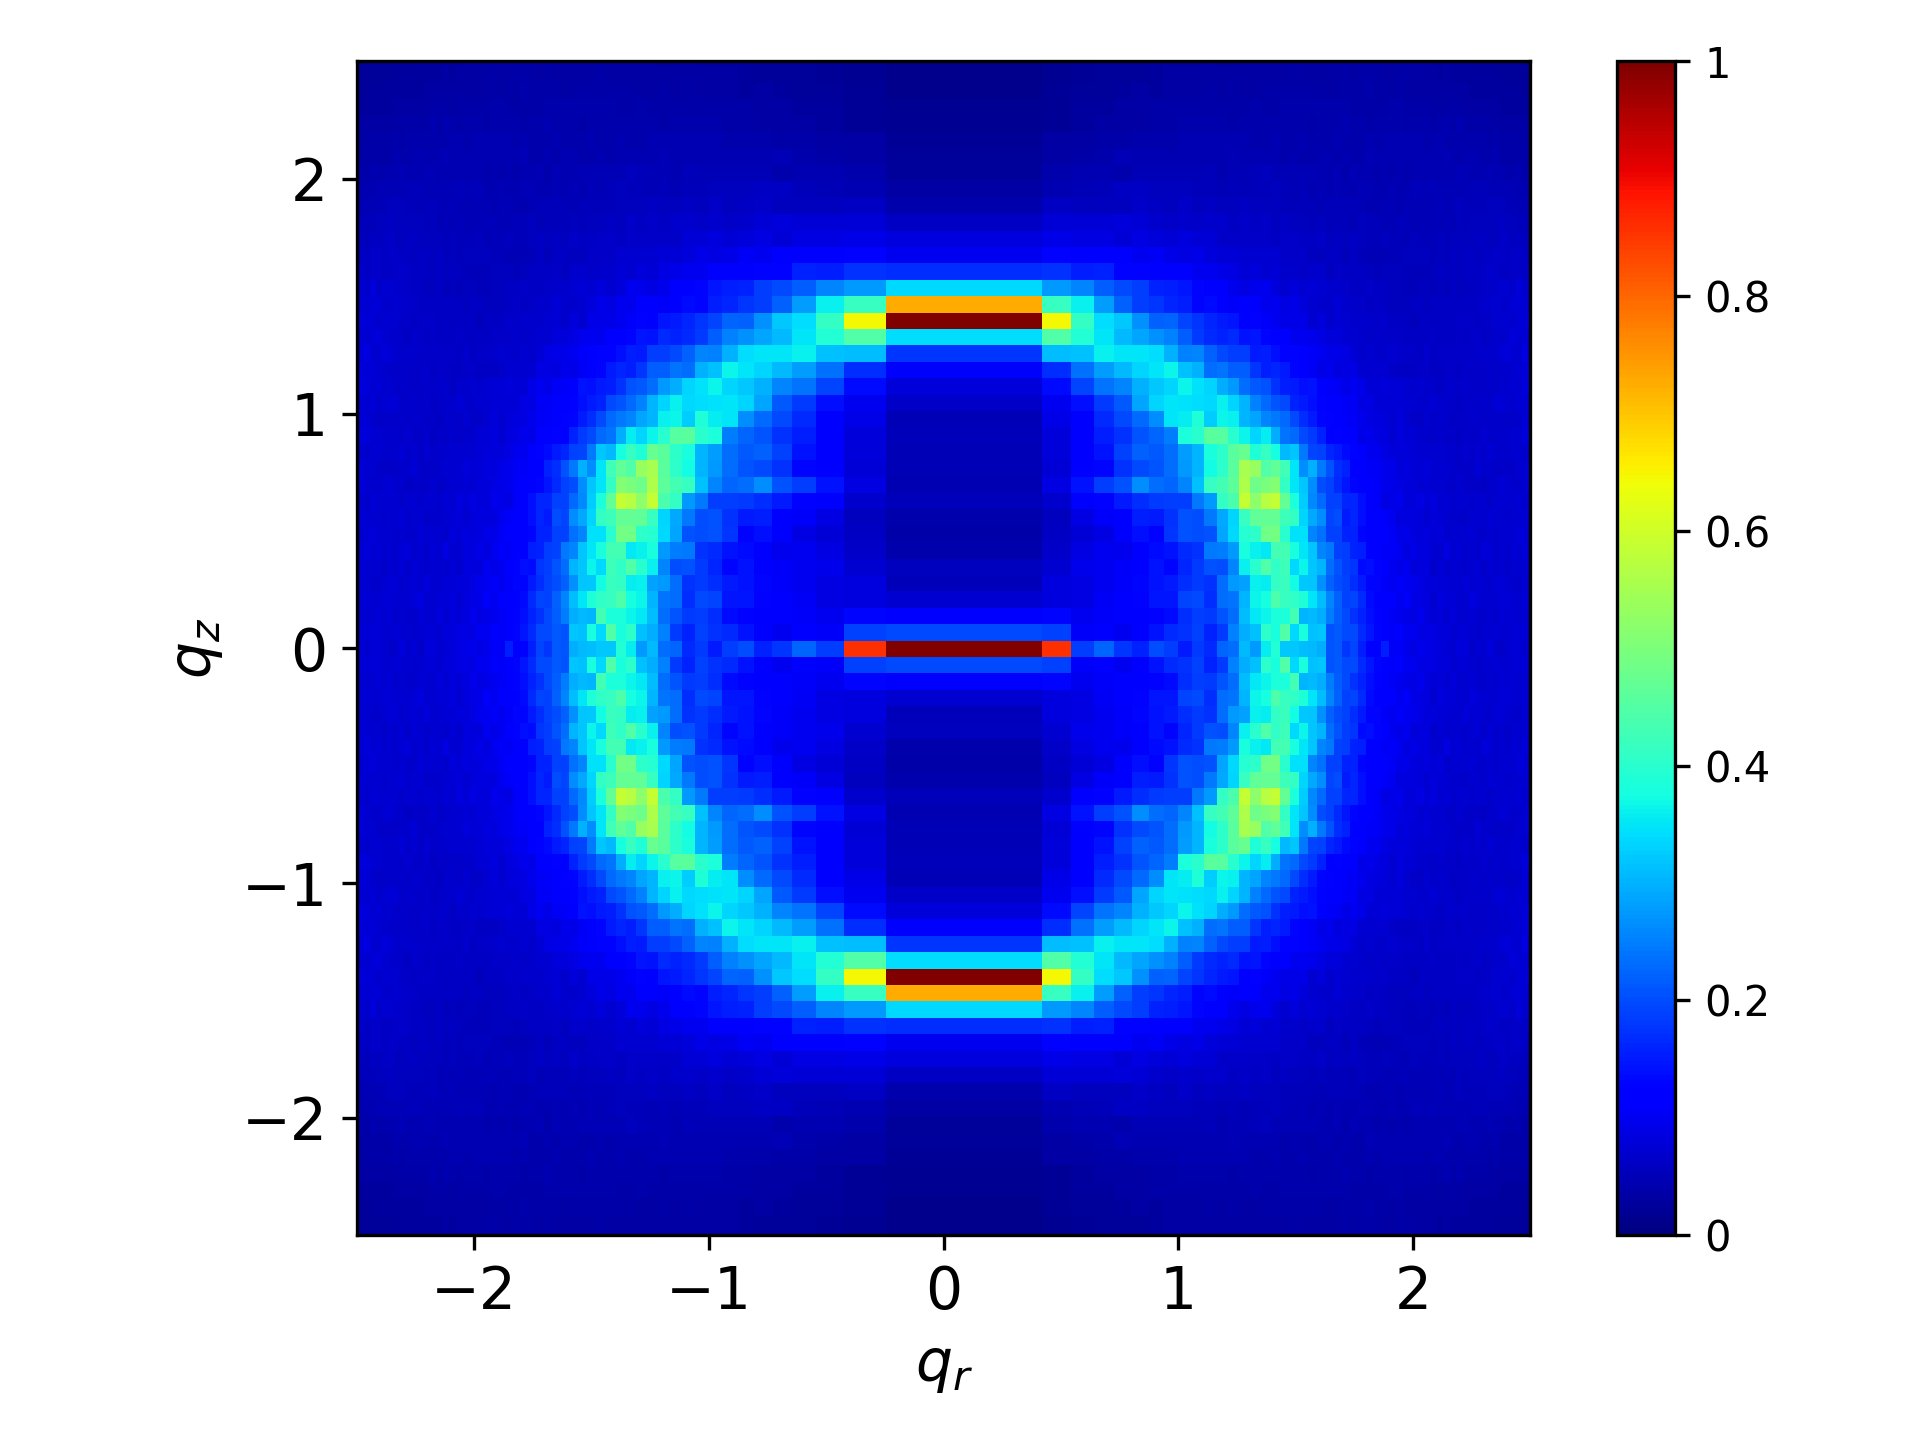
\includegraphics[width=\textwidth]{rzplot_offset_7.png}
                \caption{7 mon/layer, Parallel Displaced}\label{fig:rzplot_offset_7}
        \end{subfigure}
        \begin{subfigure}{0.40\textwidth}
                \centering
                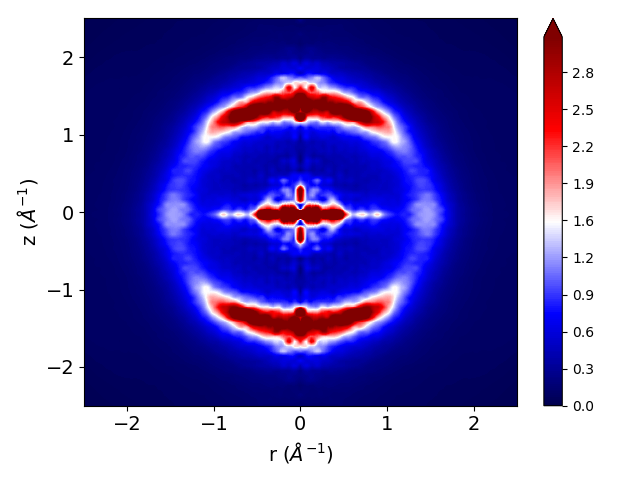
\includegraphics[width=\textwidth]{rzplot_layered_8.png}
                \caption{8 mon/layer, Sandwiched}\label{fig:rzplot_layered_8}
        \end{subfigure}
        \begin{subfigure}{0.40\textwidth}
                \centering
                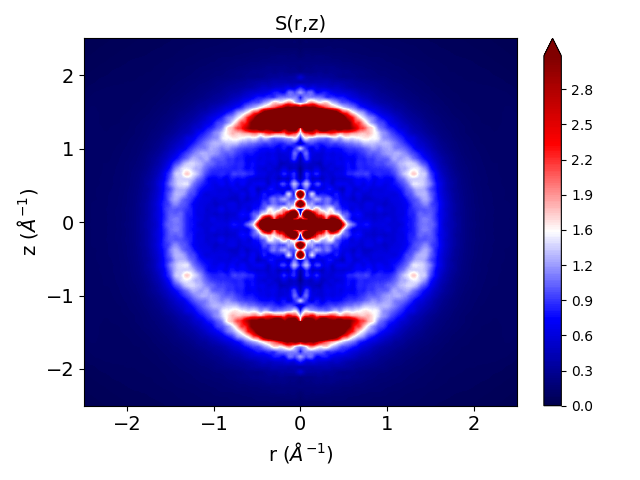
\includegraphics[width=\textwidth]{rzplot_offset_8.png}
                \caption{8 mon/layer, Parallel Displaced}\label{fig:rzplot_offset_8}
        \end{subfigure}
	\caption{Simulated XRD patterns for all other configurations built with
		 layers stacked 3.7 \AA~apart}\label{fig:XRDsim}
  \end{figure}

%  \begin{wrapfigure}{R}{0.4\textwidth}
%      \centering
%      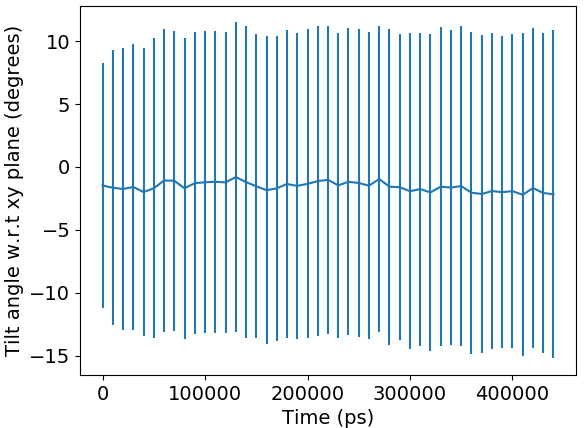
\includegraphics[width=0.4\textwidth]{tilt.png}
%      \caption{The average angle between alkane chains and the xy plane is nearly zero degrees}\label{fig:tilt}     
%  \end{wrapfigure}


%  \begin{figure}
%	\centering
%	\begin{subfigure}{0.45\textwidth}
%		\centering
%		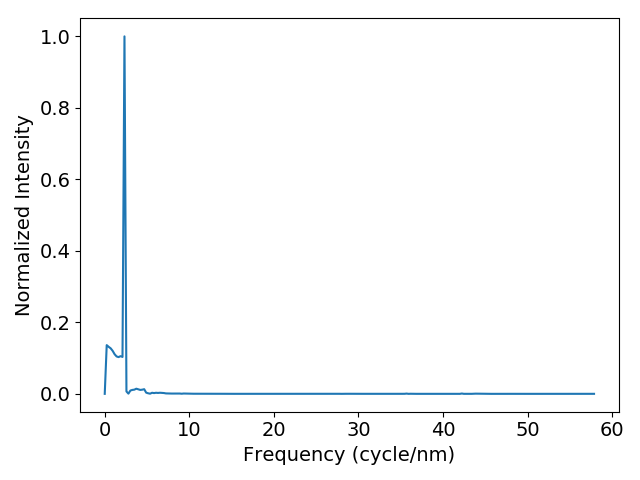
\includegraphics[width=\textwidth]{ps5layered.png}
%		\caption{}\label(fig:ps5layered}
%	\end{subfigure}
%	\begin{subfigure}
%		\centering
%		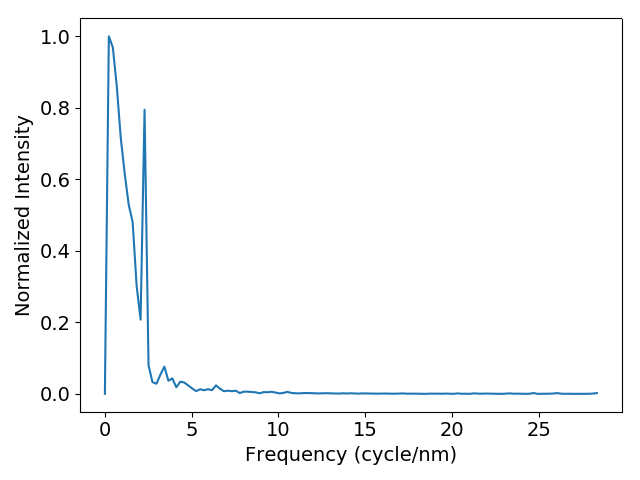
\includegraphics[width=\textwidth]{ps5offset.png}
%		\caption{}\label{fig:ps5offset}
%	\end{subfigure}
%  \end{figure}


  \begin{figure}[!ht]
        \centering
%        \begin{subfigure}{0.45\textwidth}
%                \centering
%                \hspace{-1cm}
%                \vspace{1cm}
%                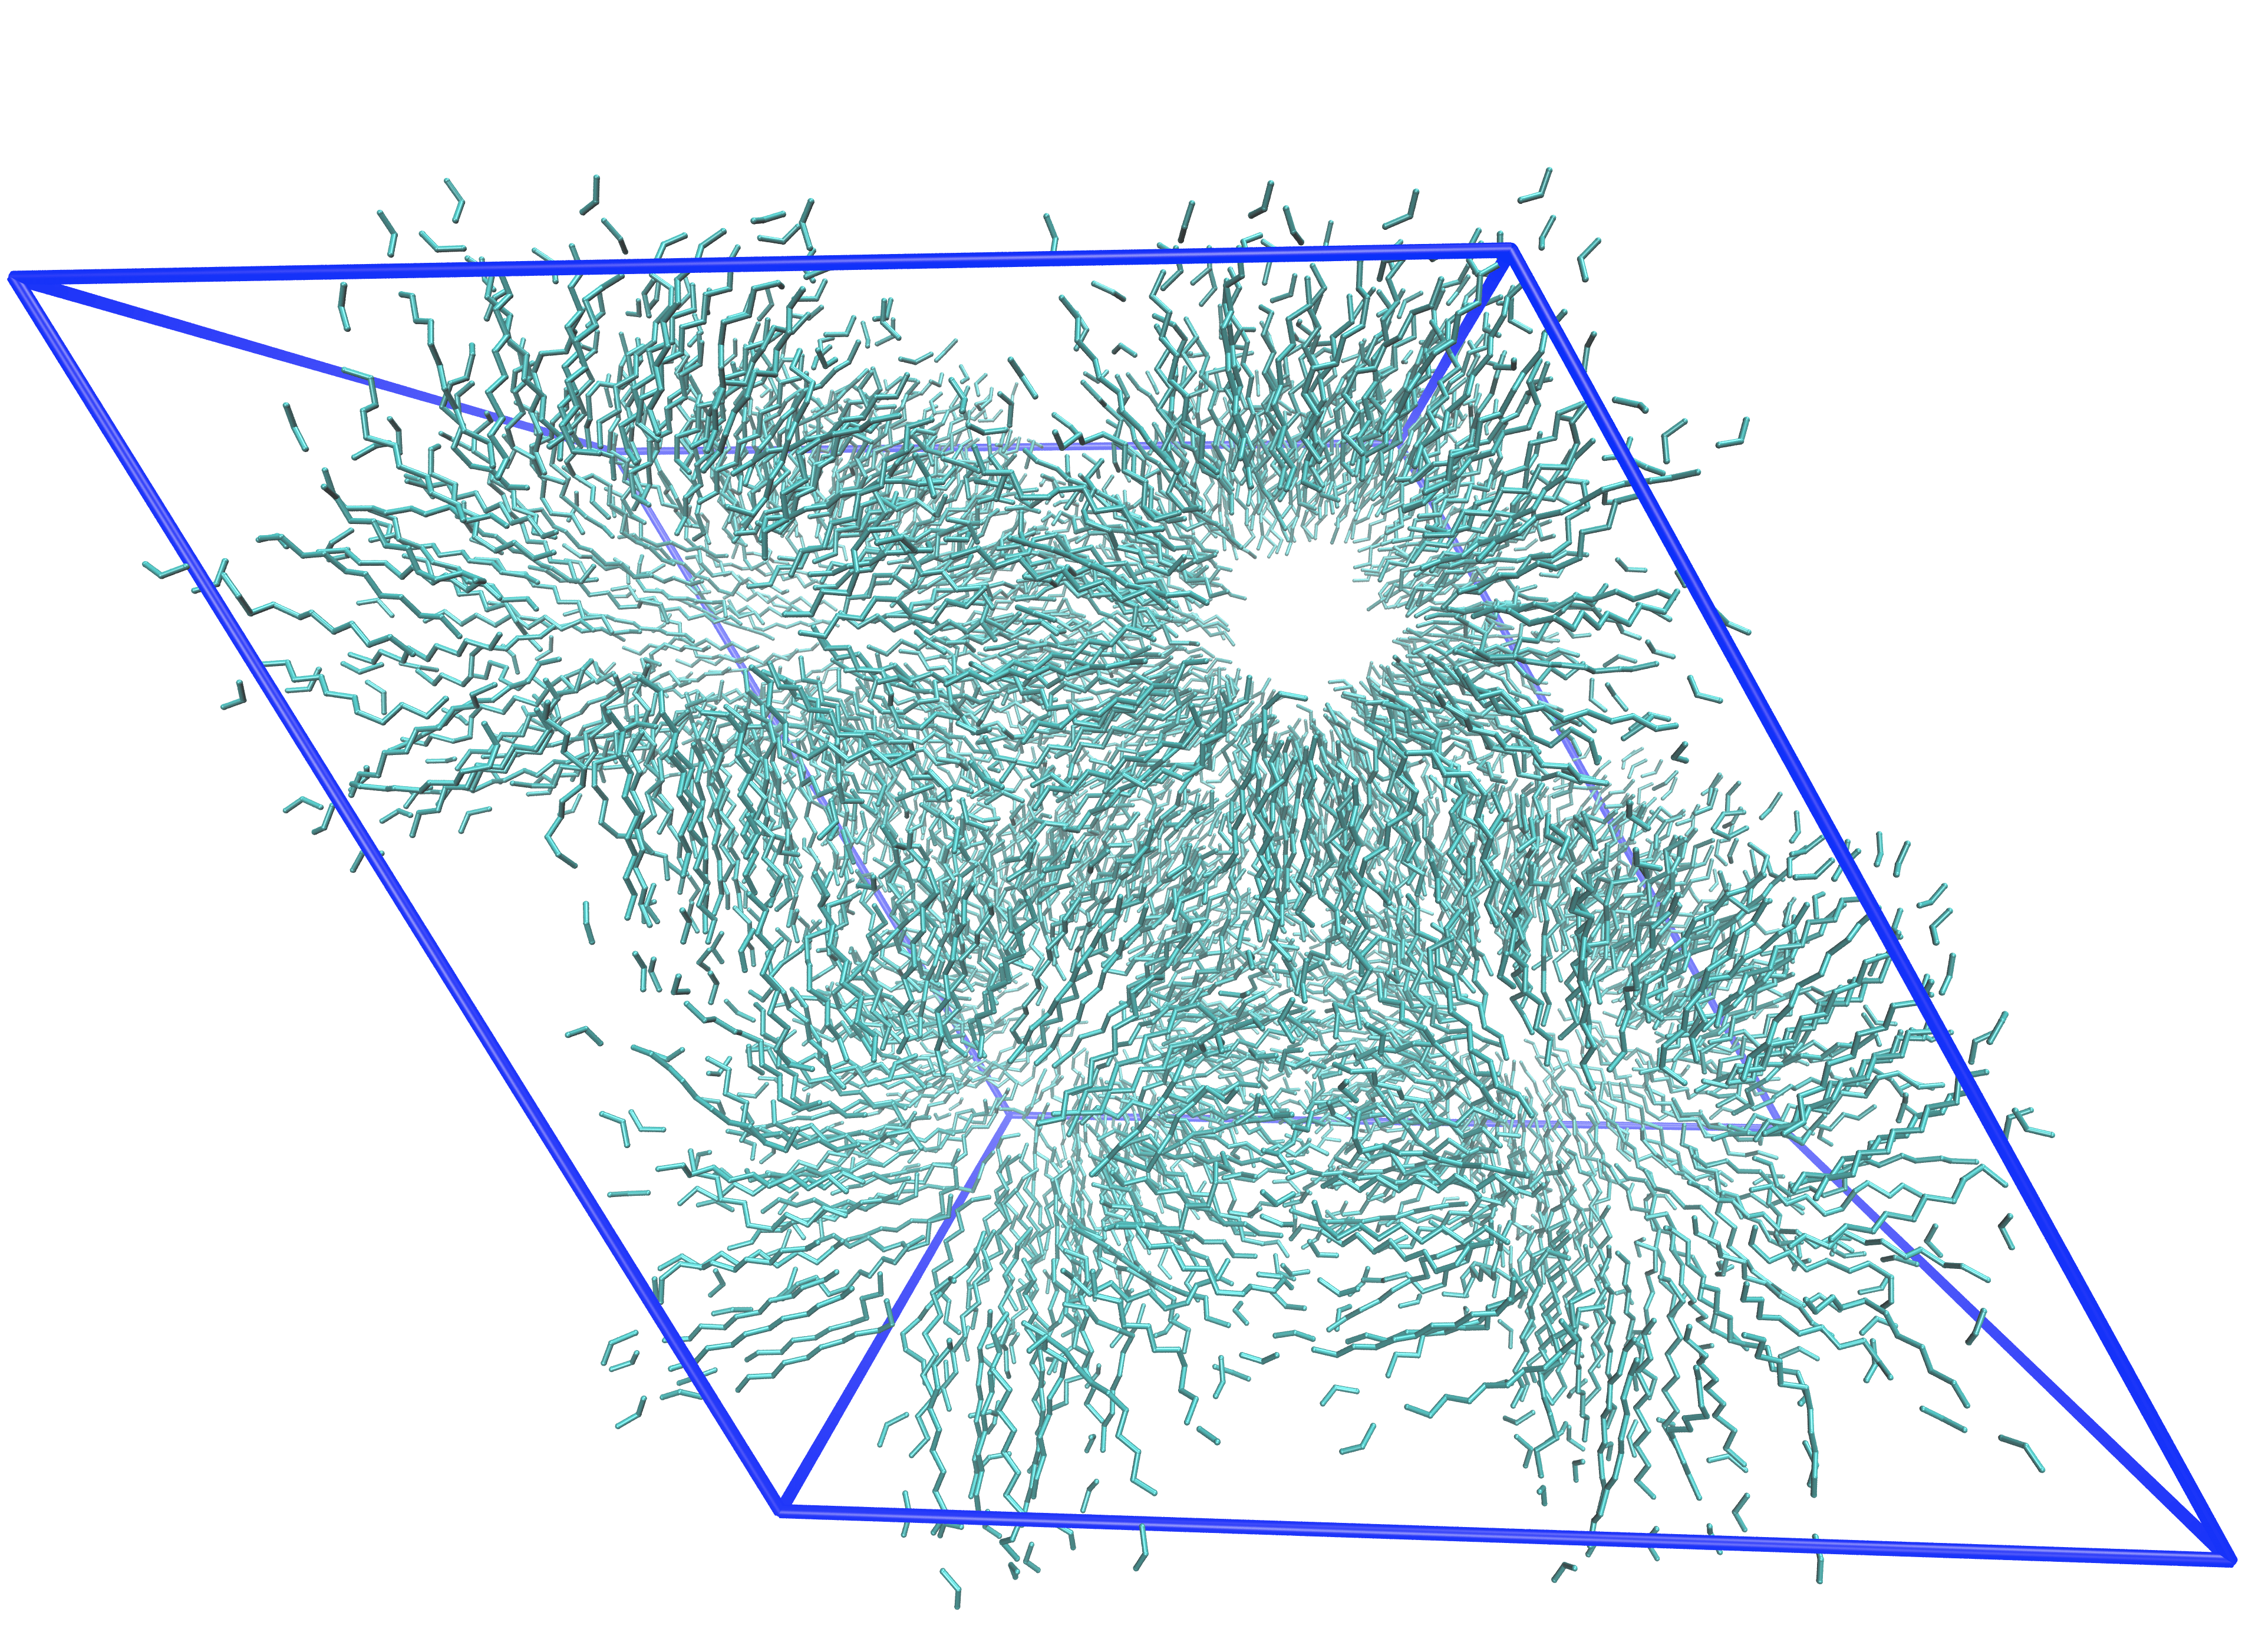
\includegraphics[width=\textwidth,scale=2]{tails_topview.png}
%                \caption{}\label{fig:tails_topview}
%        \end{subfigure}
%        \begin{subfigure}{0.45\textwidth}
%                \centering
%                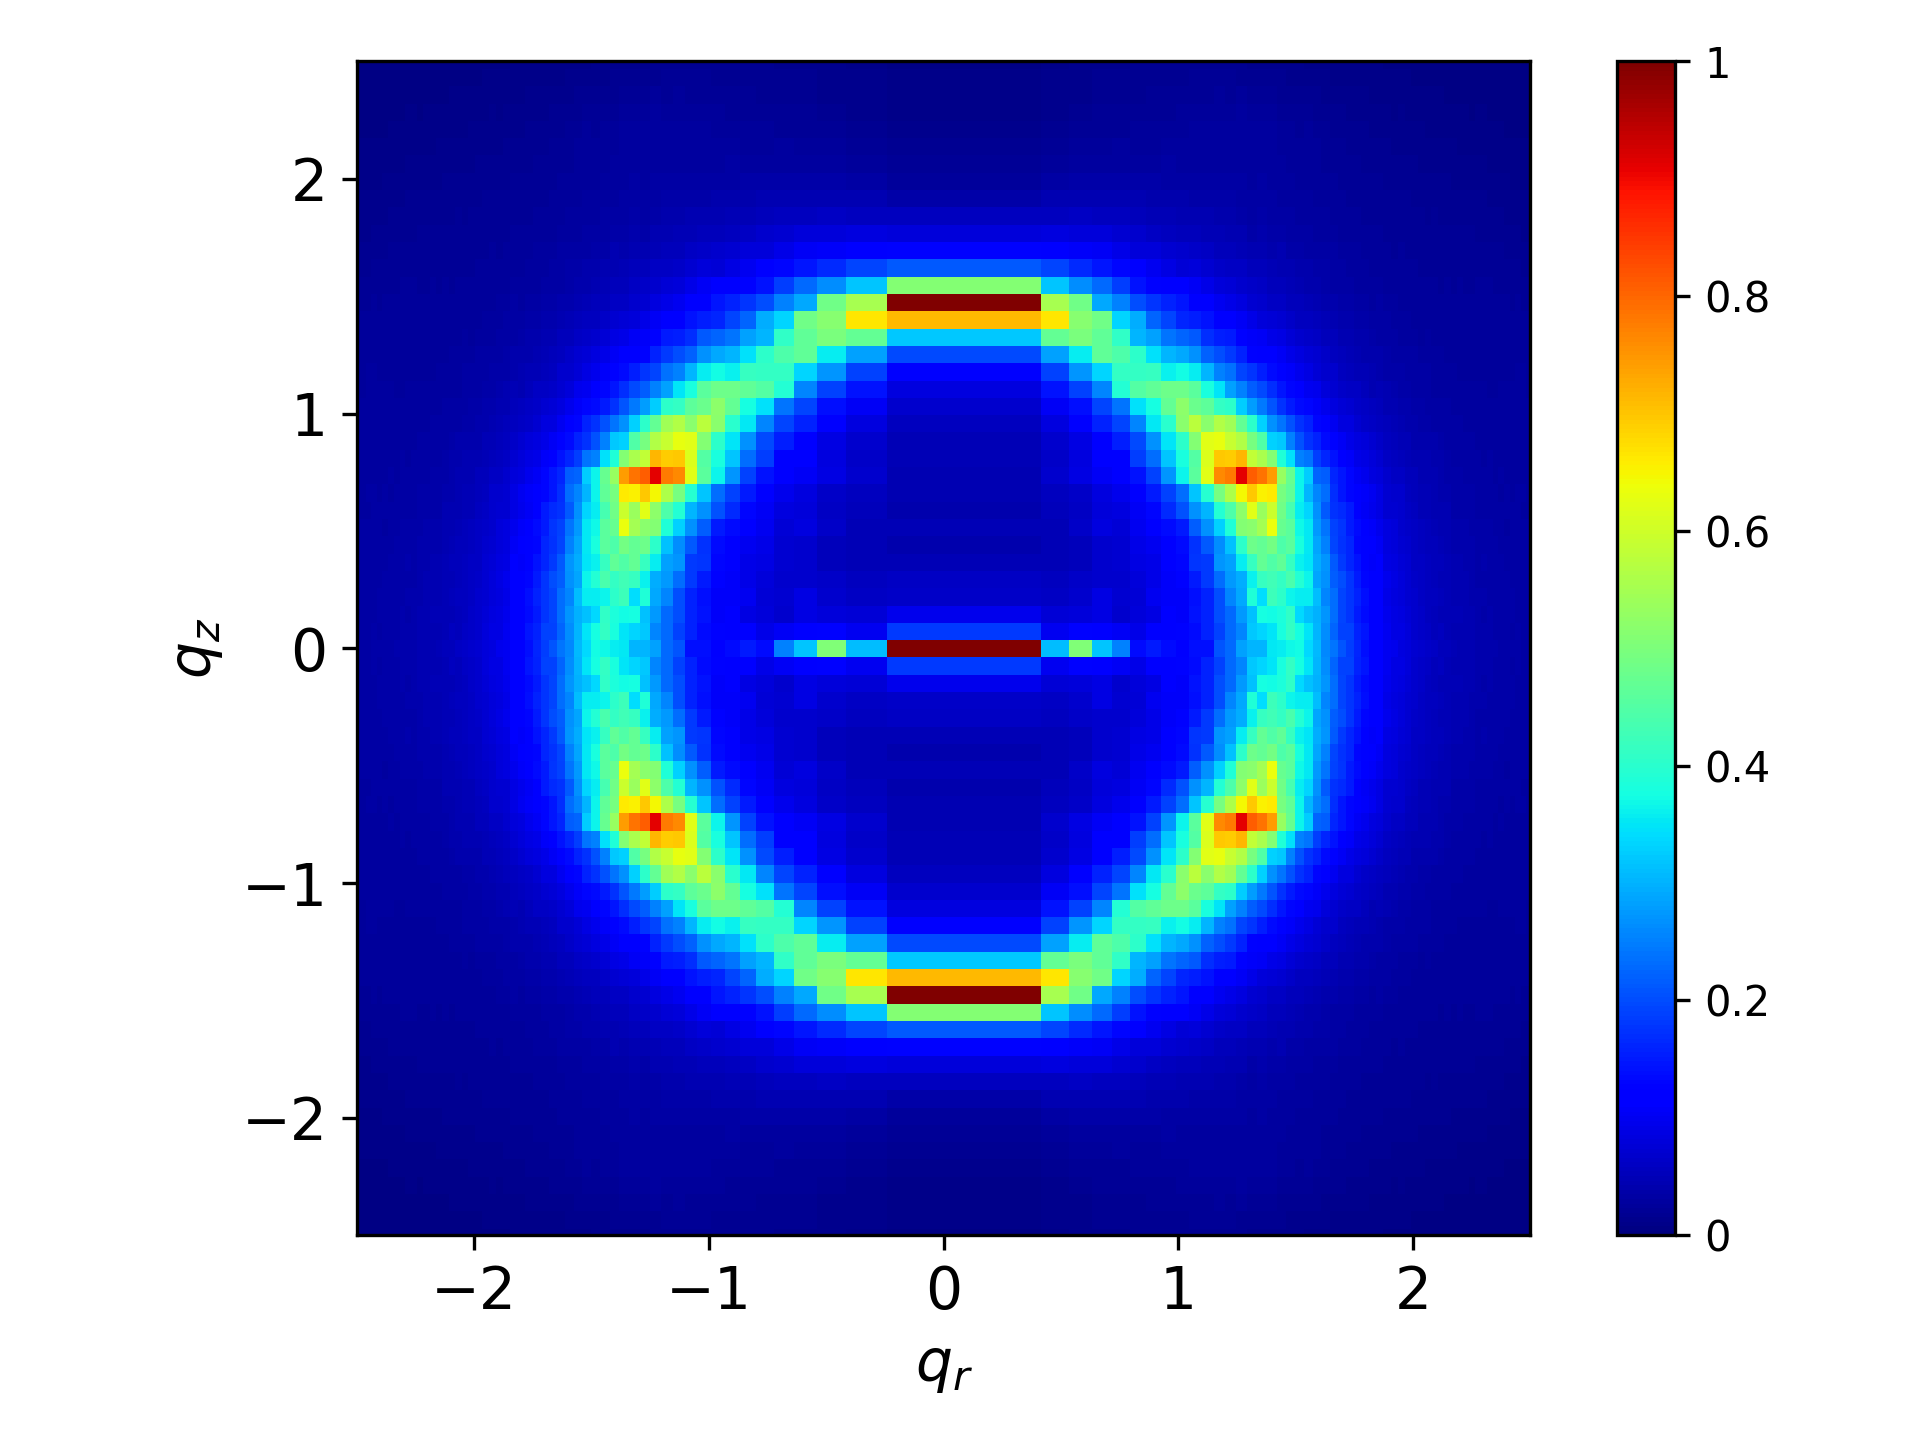
\includegraphics[width=\textwidth]{tails_rzplot.png}
%                \caption{}\label{fig:tails_rzplot}
%        \end{subfigure}
%        \begin{subfigure}{0.45\textwidth}
                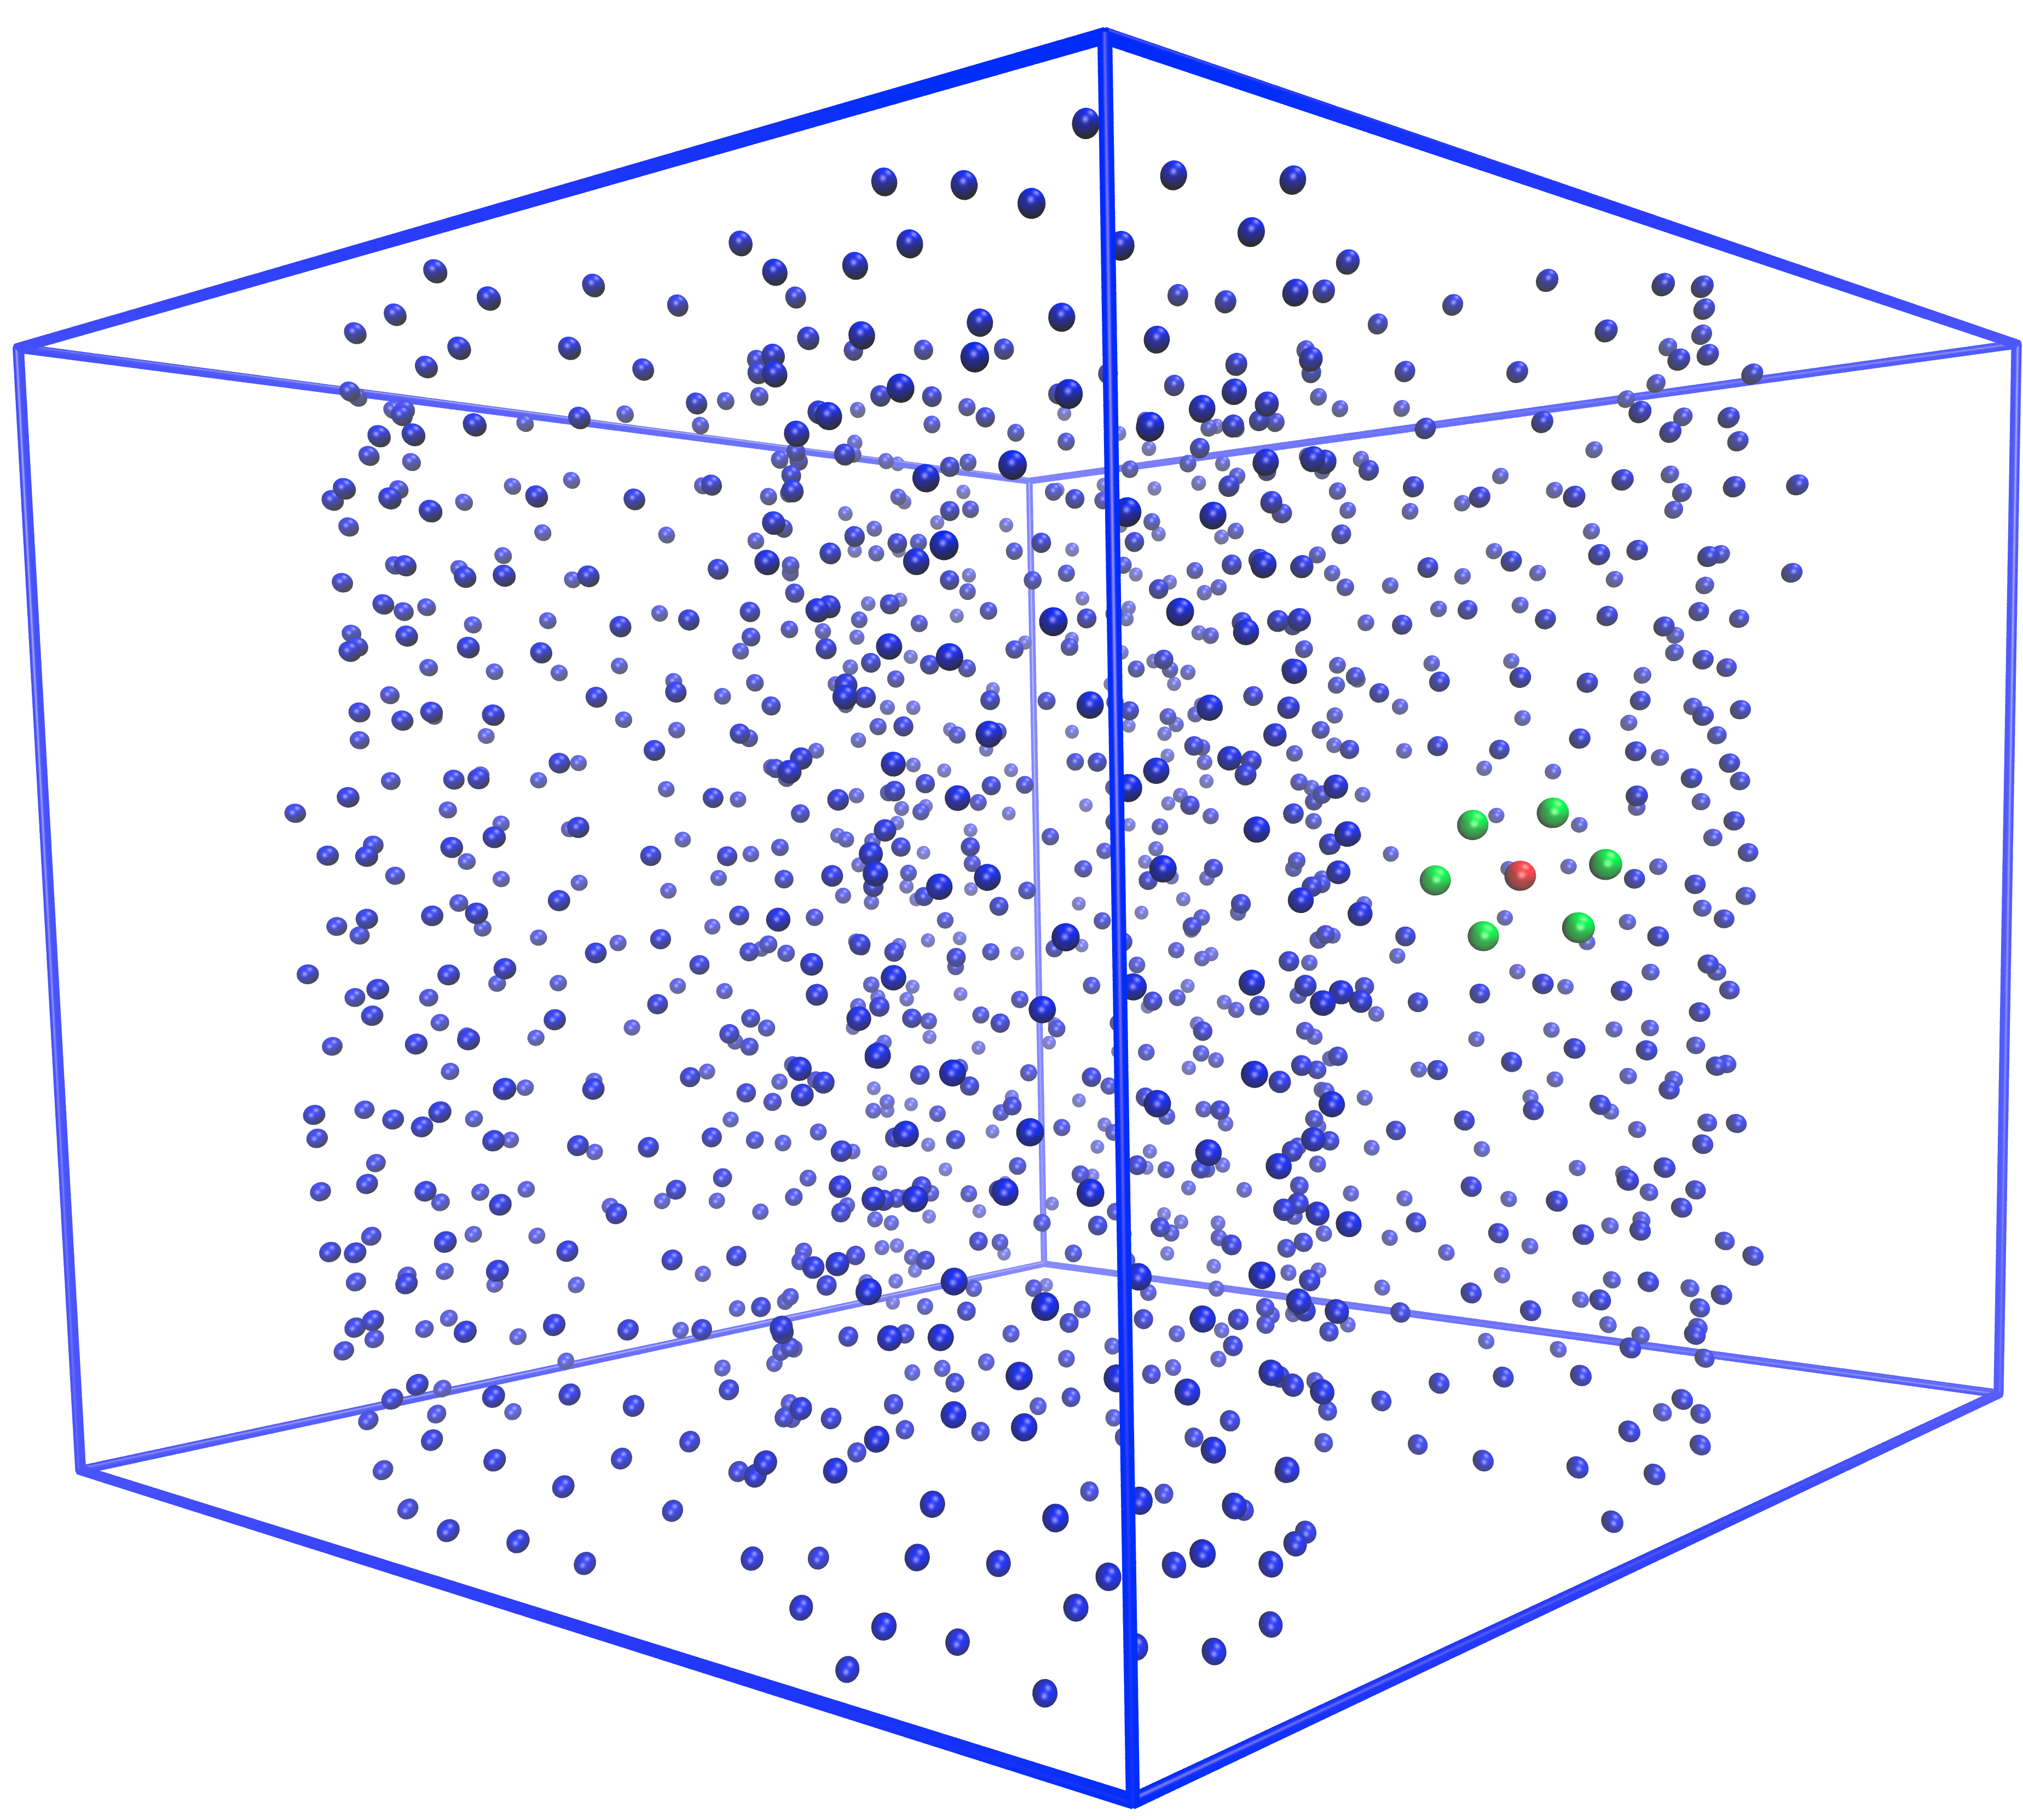
\includegraphics[width=0.5\textwidth]{centroids_box.png}
		\caption{Monomer tails pack together hexagonally. The centroid
			of each tail is visualized as a blue sphere. The centroids are calculated based
			on the red atoms in Figure~\ref{fig:monomer_color_coded}. The red sphere
			highlights an example of an alkane tail centroid with its nearest neighbors
			(green spheres) surrounding it in a hexagonal pattern.}\label{fig:centroids}
%        \end{subfigure}
%        \begin{subfigure}{0.45\textwidth}
%                \centering
%                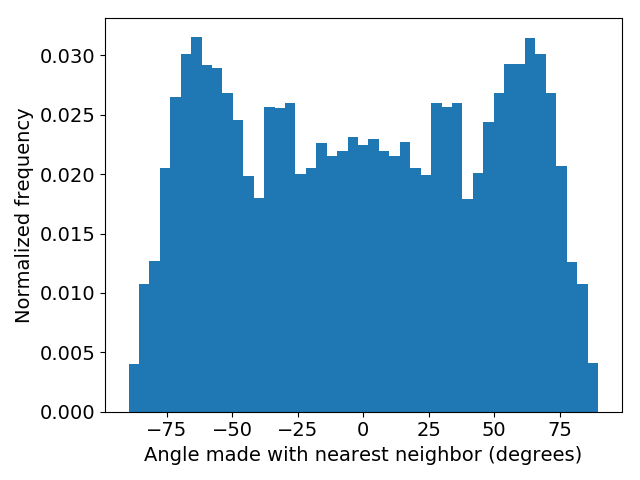
\includegraphics[width=\textwidth]{angles_traj_layered.png}
%                \caption{}\label{fig:angle_distribution}
%        \end{subfigure}
%        \caption{(a) The trajectory can be stripped of all atoms except carbon
%        atoms in monomer tails. (b) Simulated diffraction of the tail-only trajectory
%        still gives rise to R-spots. (c) Finding the center of mass and visualizing
%        their coordinates reveals the hexagonal-like packing of the tails. (d) The
%        distribution created by measuring the angle between each centroid (e.g. red
%        in (c)) and its neareset neighbors (e.g. green in (c)) with respect to the xy
%        plane has distinct spikes near 30\degree, which is consistent with the location
%        of R-spots}\label{fig:tail_packing}
  \end{figure}

  \begin{figure}
  \centering
        \begin{subfigure}{0.45\textwidth}
                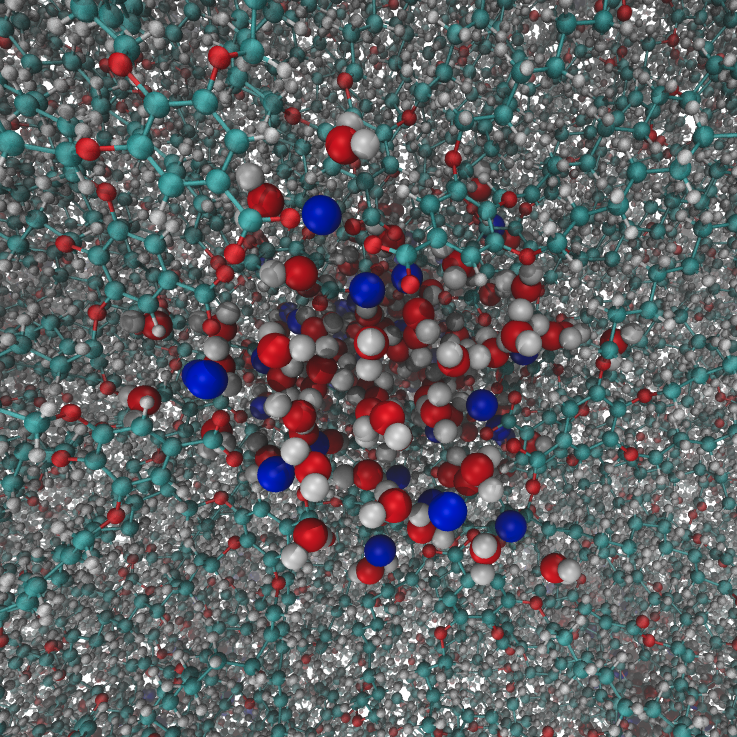
\includegraphics[width=\textwidth]{water_filled_pore.png}
                \caption{}\label{fig:water_filled_pores}
        \end{subfigure}
        \begin{subfigure}{0.45\textwidth}
                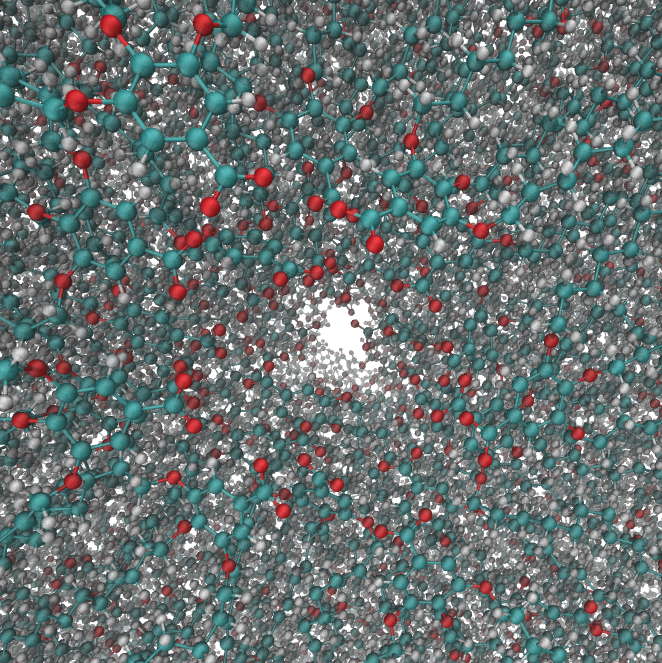
\includegraphics[width=\textwidth]{water_removed.png}
                \caption{}\label{fig:water_removed}
        \end{subfigure}
  \caption{(a) Pores built in the parallel displaced configuration with 5
	  monomers per layer are filled with 5 wt\% water. (b) The same system is
	  visualized with water molecules and sodium ions removed. Head groups vacate the
	  pore region leaving an aqeuous solution of water and sodium ions.}\label{fig:water_pores}
  \end{figure}

\end{document}
